\documentclass[../DD.tex]{subfiles}
\graphicspath{{\subfix{../assets}}}

\usepackage{geometry}

\begin{document}
    \subsection{Overview}\label{subsec:overview}
    The system's architecture is organized in \textit{three logical layers} following the \textit{client-server} paradigm.
    \begin{figure}[H]
        \centering
        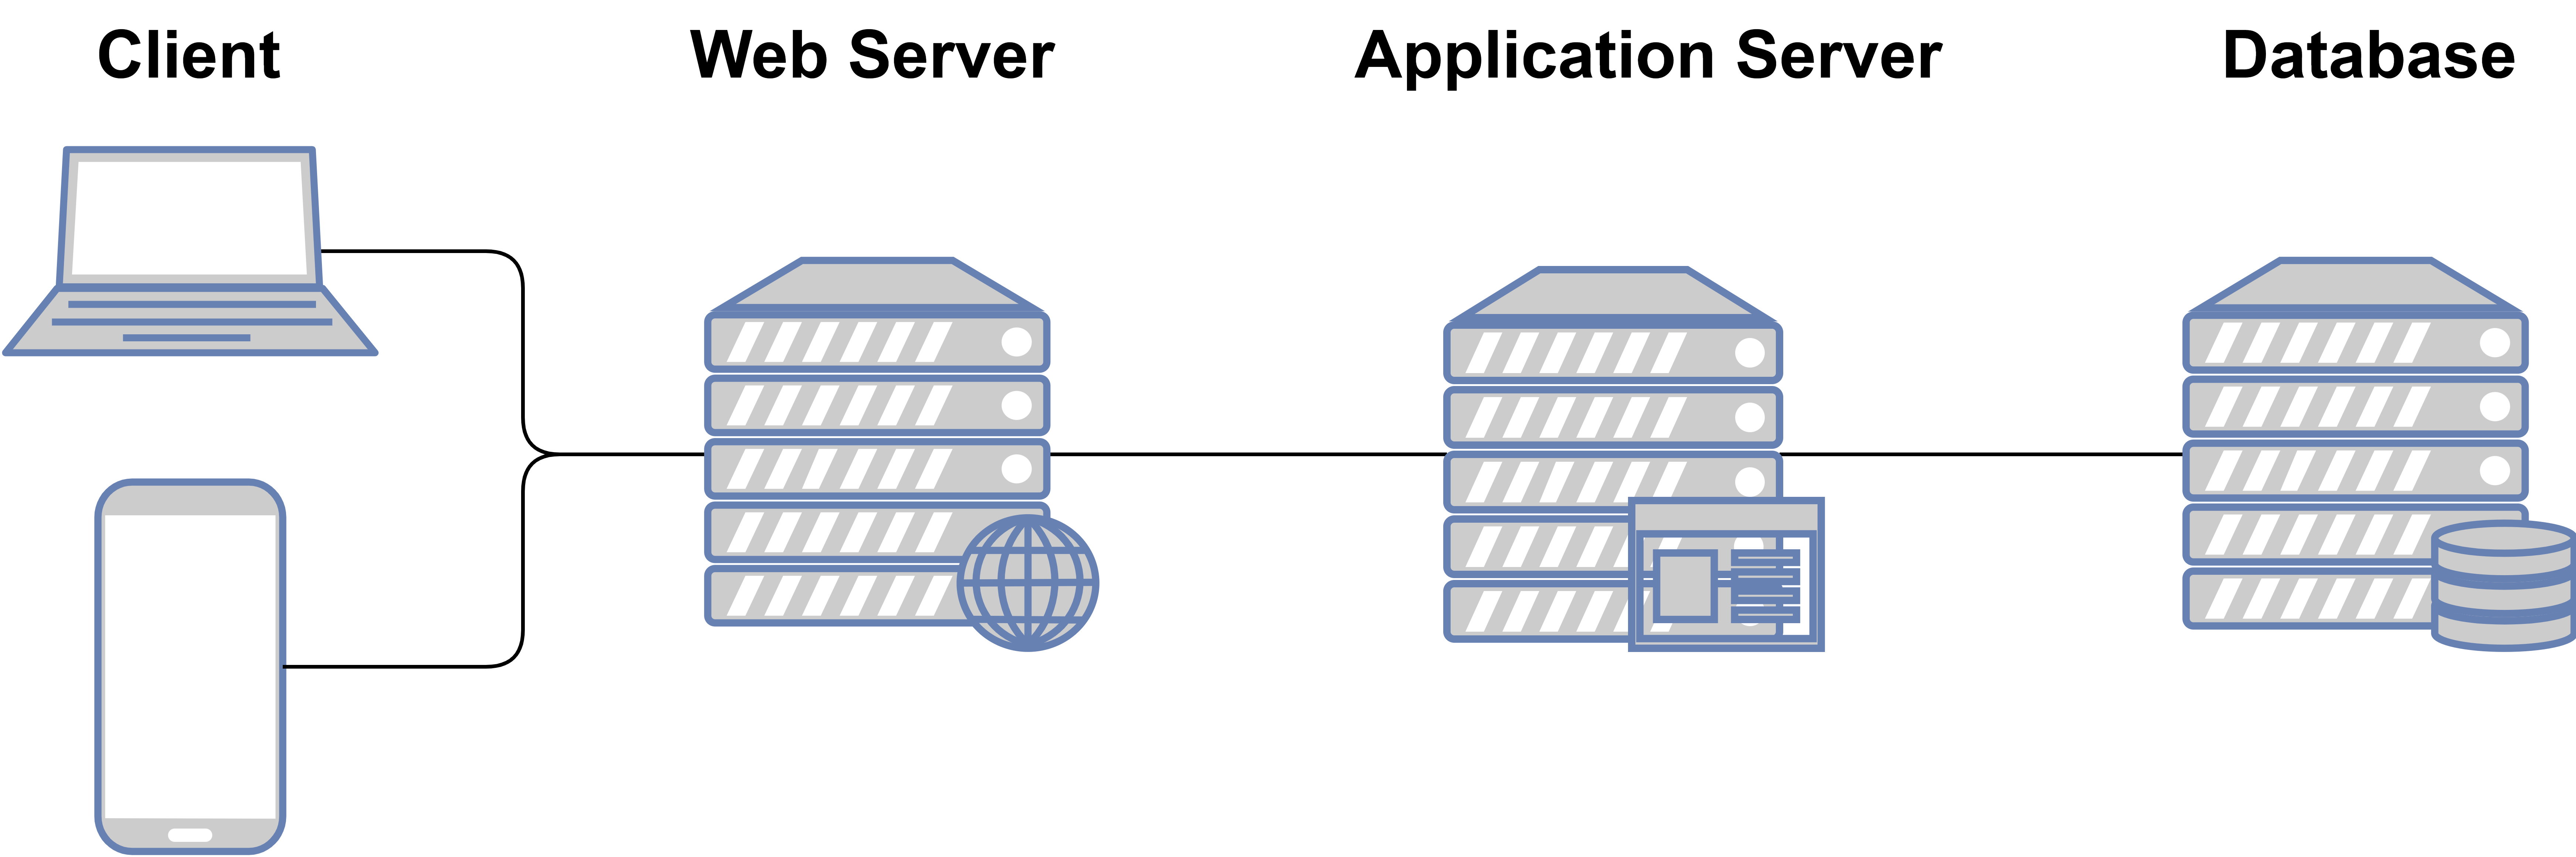
\includegraphics[width=\textwidth]{../assets/section_2/3-tier-architecture.png}
        \caption{Three Tier Architecture (and the clients)}
        \label{fig:3_tier_architecture}
    \end{figure}
    \begin{itemize}
        \item {\textbf{Presentation Layer (P)}: This layer is tasked with presenting the application's user interface to the client via the Web Server. 
        It is represented by a GUI designed to facilitate efficient and comfortable user interaction with the application.}
        \item {\textbf{Application Layer (A)}: The Application Layer handles the business logic of the application. 
        It receives requests from the Presentation Layer, processes them, and then sends back the results to be displayed(to the presentation layer again).}
        \item {\textbf{Data Layer (D)}: Responsible for accessing and managing data sources, the Data Layer provides data through some database and directs it to the other layers. 
        Additionally, it plays a crucial role in ensuring a high level of abstraction from the database itself by providing a proper interface}
    \end{itemize}

        \subsubsection{High level architecture}\label{subsubsec:high_level_architecture}
        \begin{figure}[H]
            \centering
            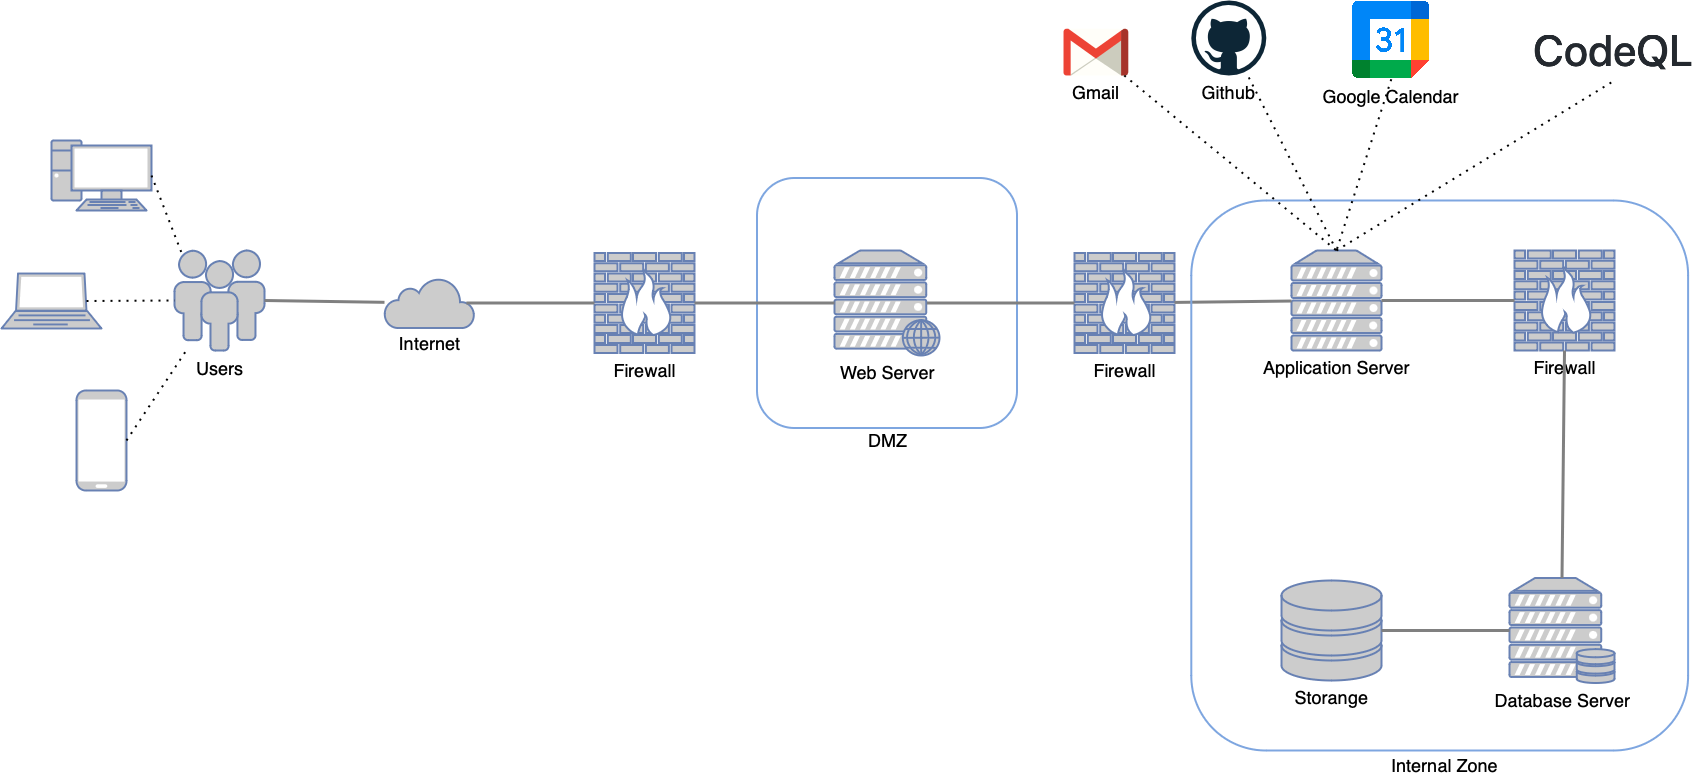
\includegraphics[width=\textwidth]{../assets/section_2/high_level_architecture.png}
            \caption{High Level Architecture}
            \label{fig:high_level_architecture}
        \end{figure}
        The figure \ref{fig:high_level_architecture} shows the high level architecture of the system.
        It's divided in two different zones:
        \begin{itemize}
            \item {\textit{Demilitarized Zone}: represent the area of the system where the system is partially exposed to the internet, hence the users.
            In this zone the \textit{Web Server} is located.
            Its primary role is to handle the communication and interaction between the whole system and the final users.}
            \item {\textit{Internal Zone}: represent the internal area of the system where the business logic and the data are located.
            Here the \textit{Application Server} and the \textit{Database Server}\footnote{The database server is furthermore protected by another firewall} are present.}
        \end{itemize}
        This division enhances the security of the system by placing the database, one of the most common target of cyberattacks, behind three different firewalls.
        Moreover, only the application server itself is allowed to directly query the database, further reducing the risk of unauthorized access.\\
        It's necessary to clarify that the application server, even if not directly exposed to the internet, has to be connected to it in order to allow communication with external services such as the GitHub APIs.

    \newpage
    \newgeometry{top = 8em}
    \subsection{Component View}\label{subsec:component_view}
        \subsubsection*{High level component view}
        \begin{figure}[ht]
            \centering
            \hspace*{-3.5cm}
            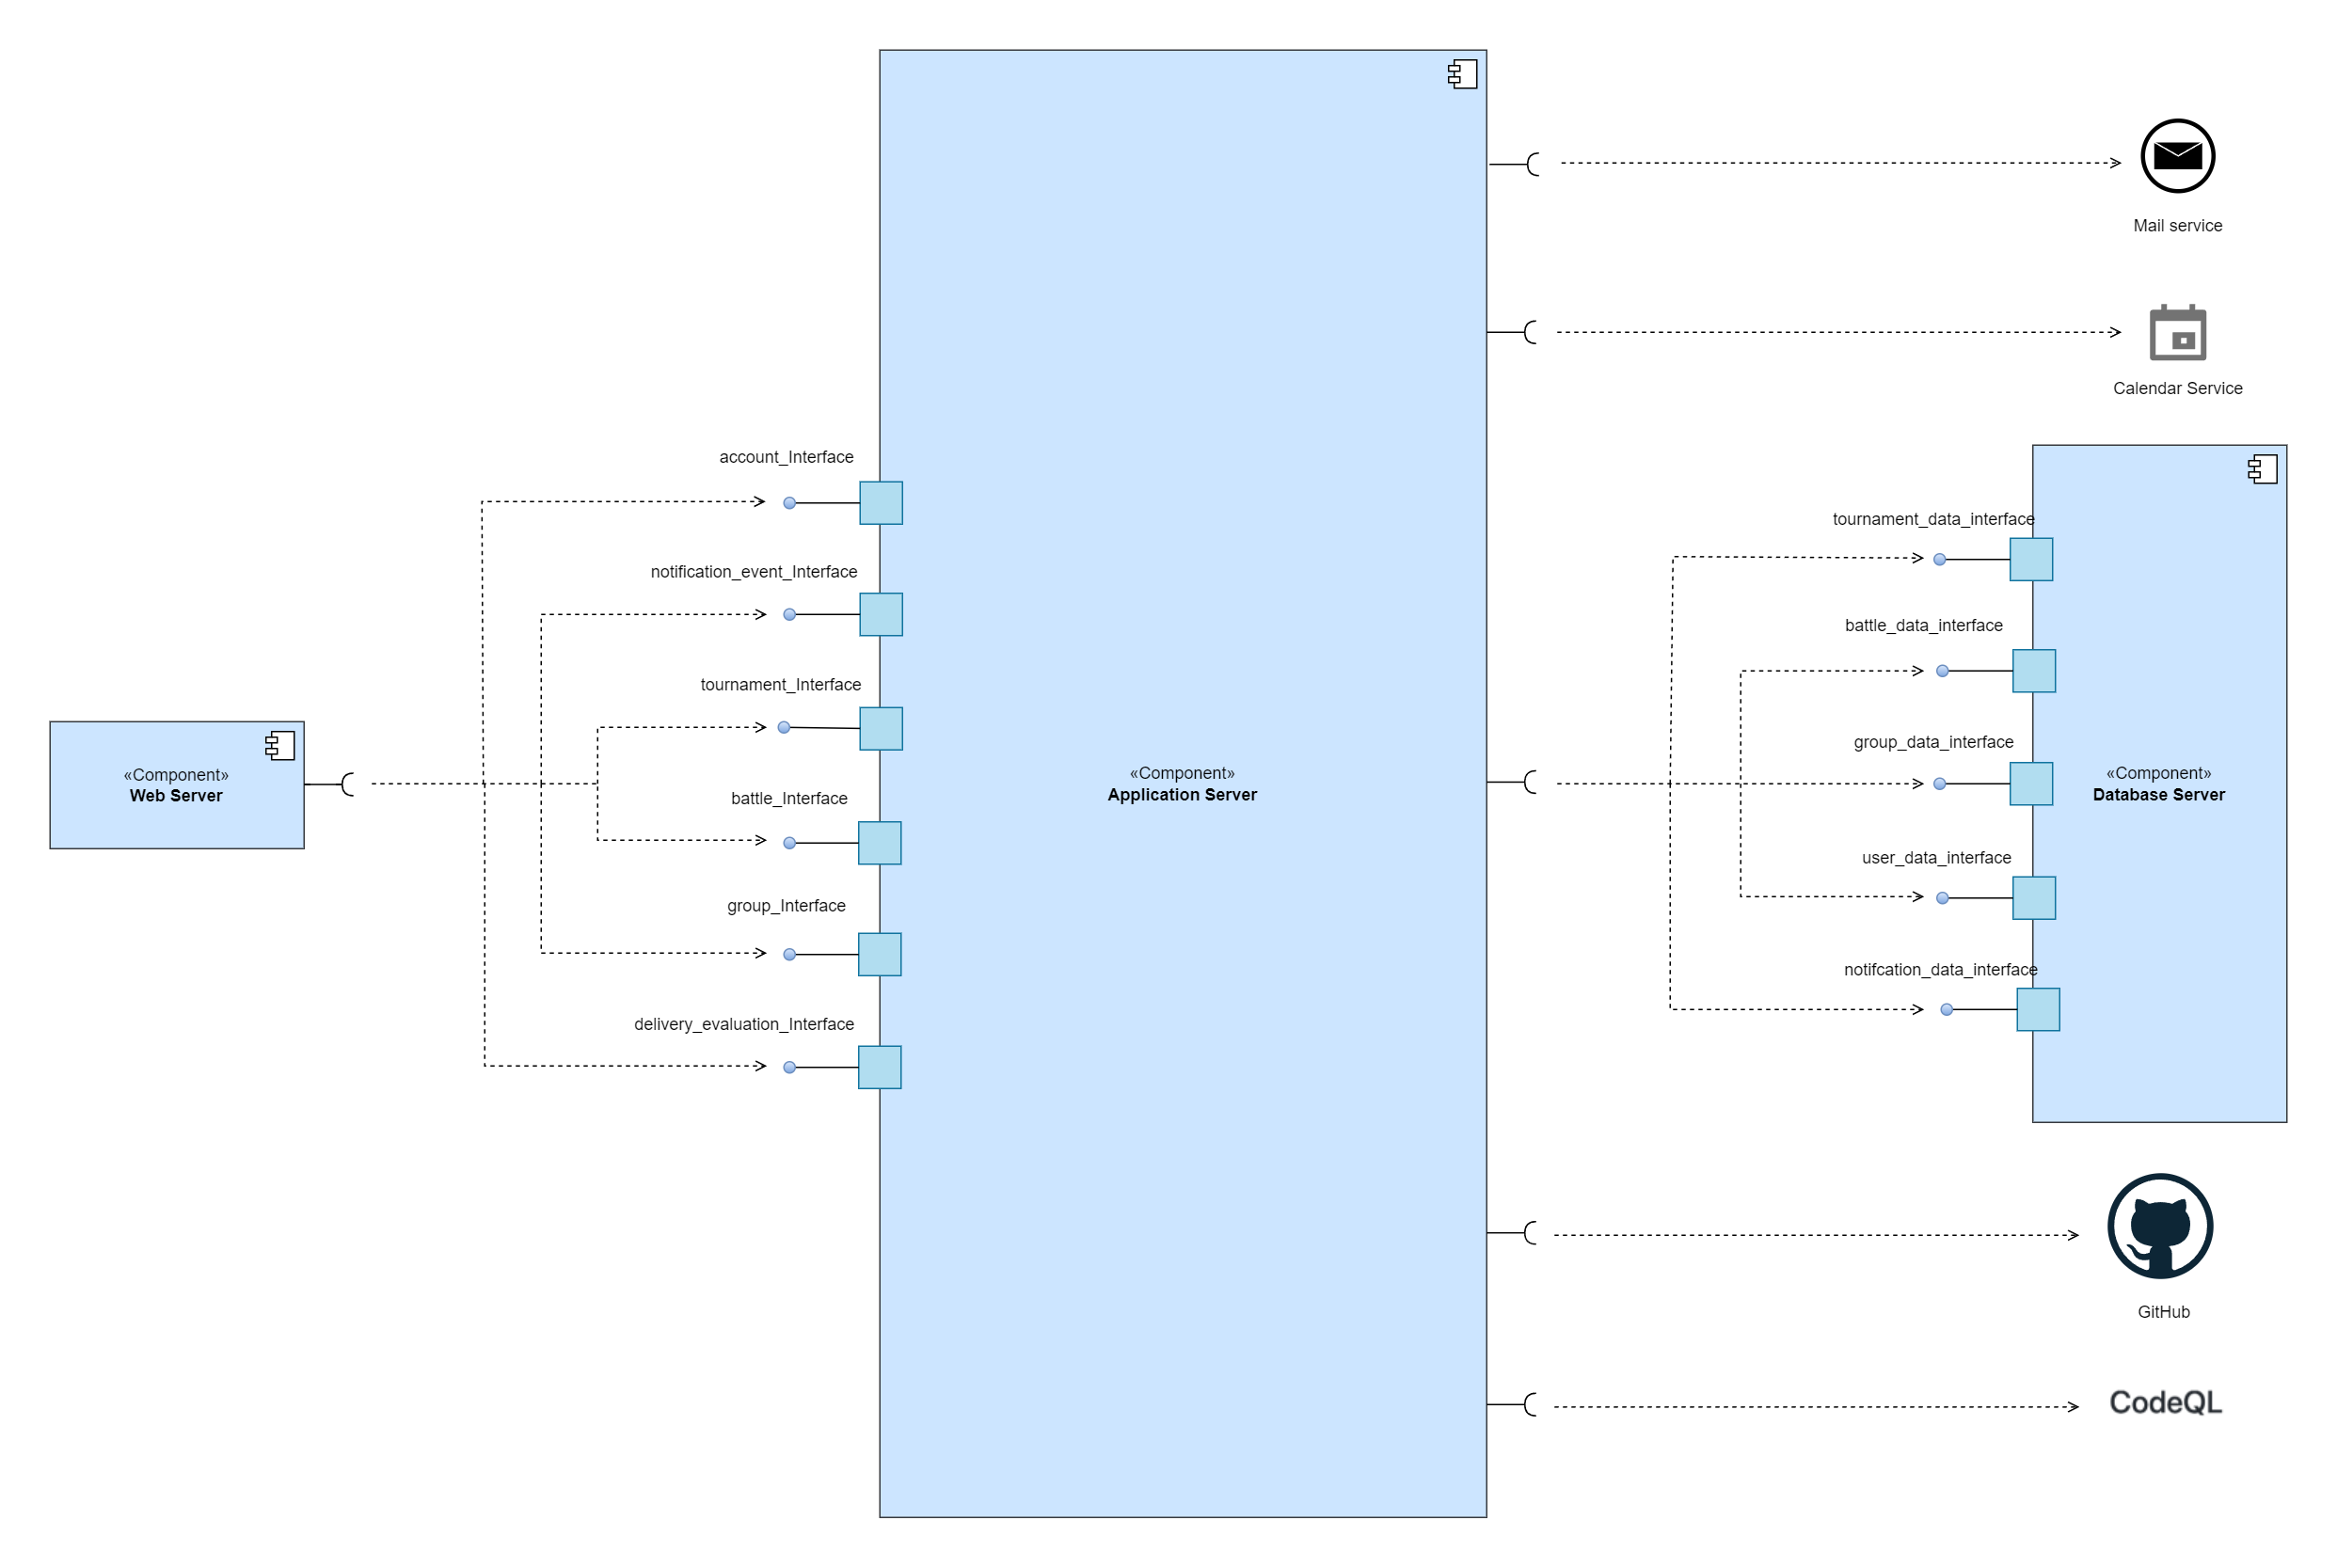
\includegraphics[width=1.4\textwidth]{../assets/section_2/HighLevelComponentDiagram.png}
        \end{figure}
        This image gives a high level representation of the components of the system, where the application server is represented as an empty box, since its complete description will be provided in the next section. The interfaces represented on the left are the ones between the web server and the system's application server, and they represent the main functionalities requested by the clients to the web server. On the opposite side the external interfaces used by the application server are presented instead, which are for example the online repository system used by CodeKata (GitHub), but also the DBMS interfaces, which are managed by the system's DBMS service and handle all the system requests for data from its external database
    \newpage
    \restoregeometry

    \newgeometry{top = 8em}
    \subsubsection*{Application server's component view}
        \begin{figure}[h!]
            \centering
            \hspace*{-3.5cm}
            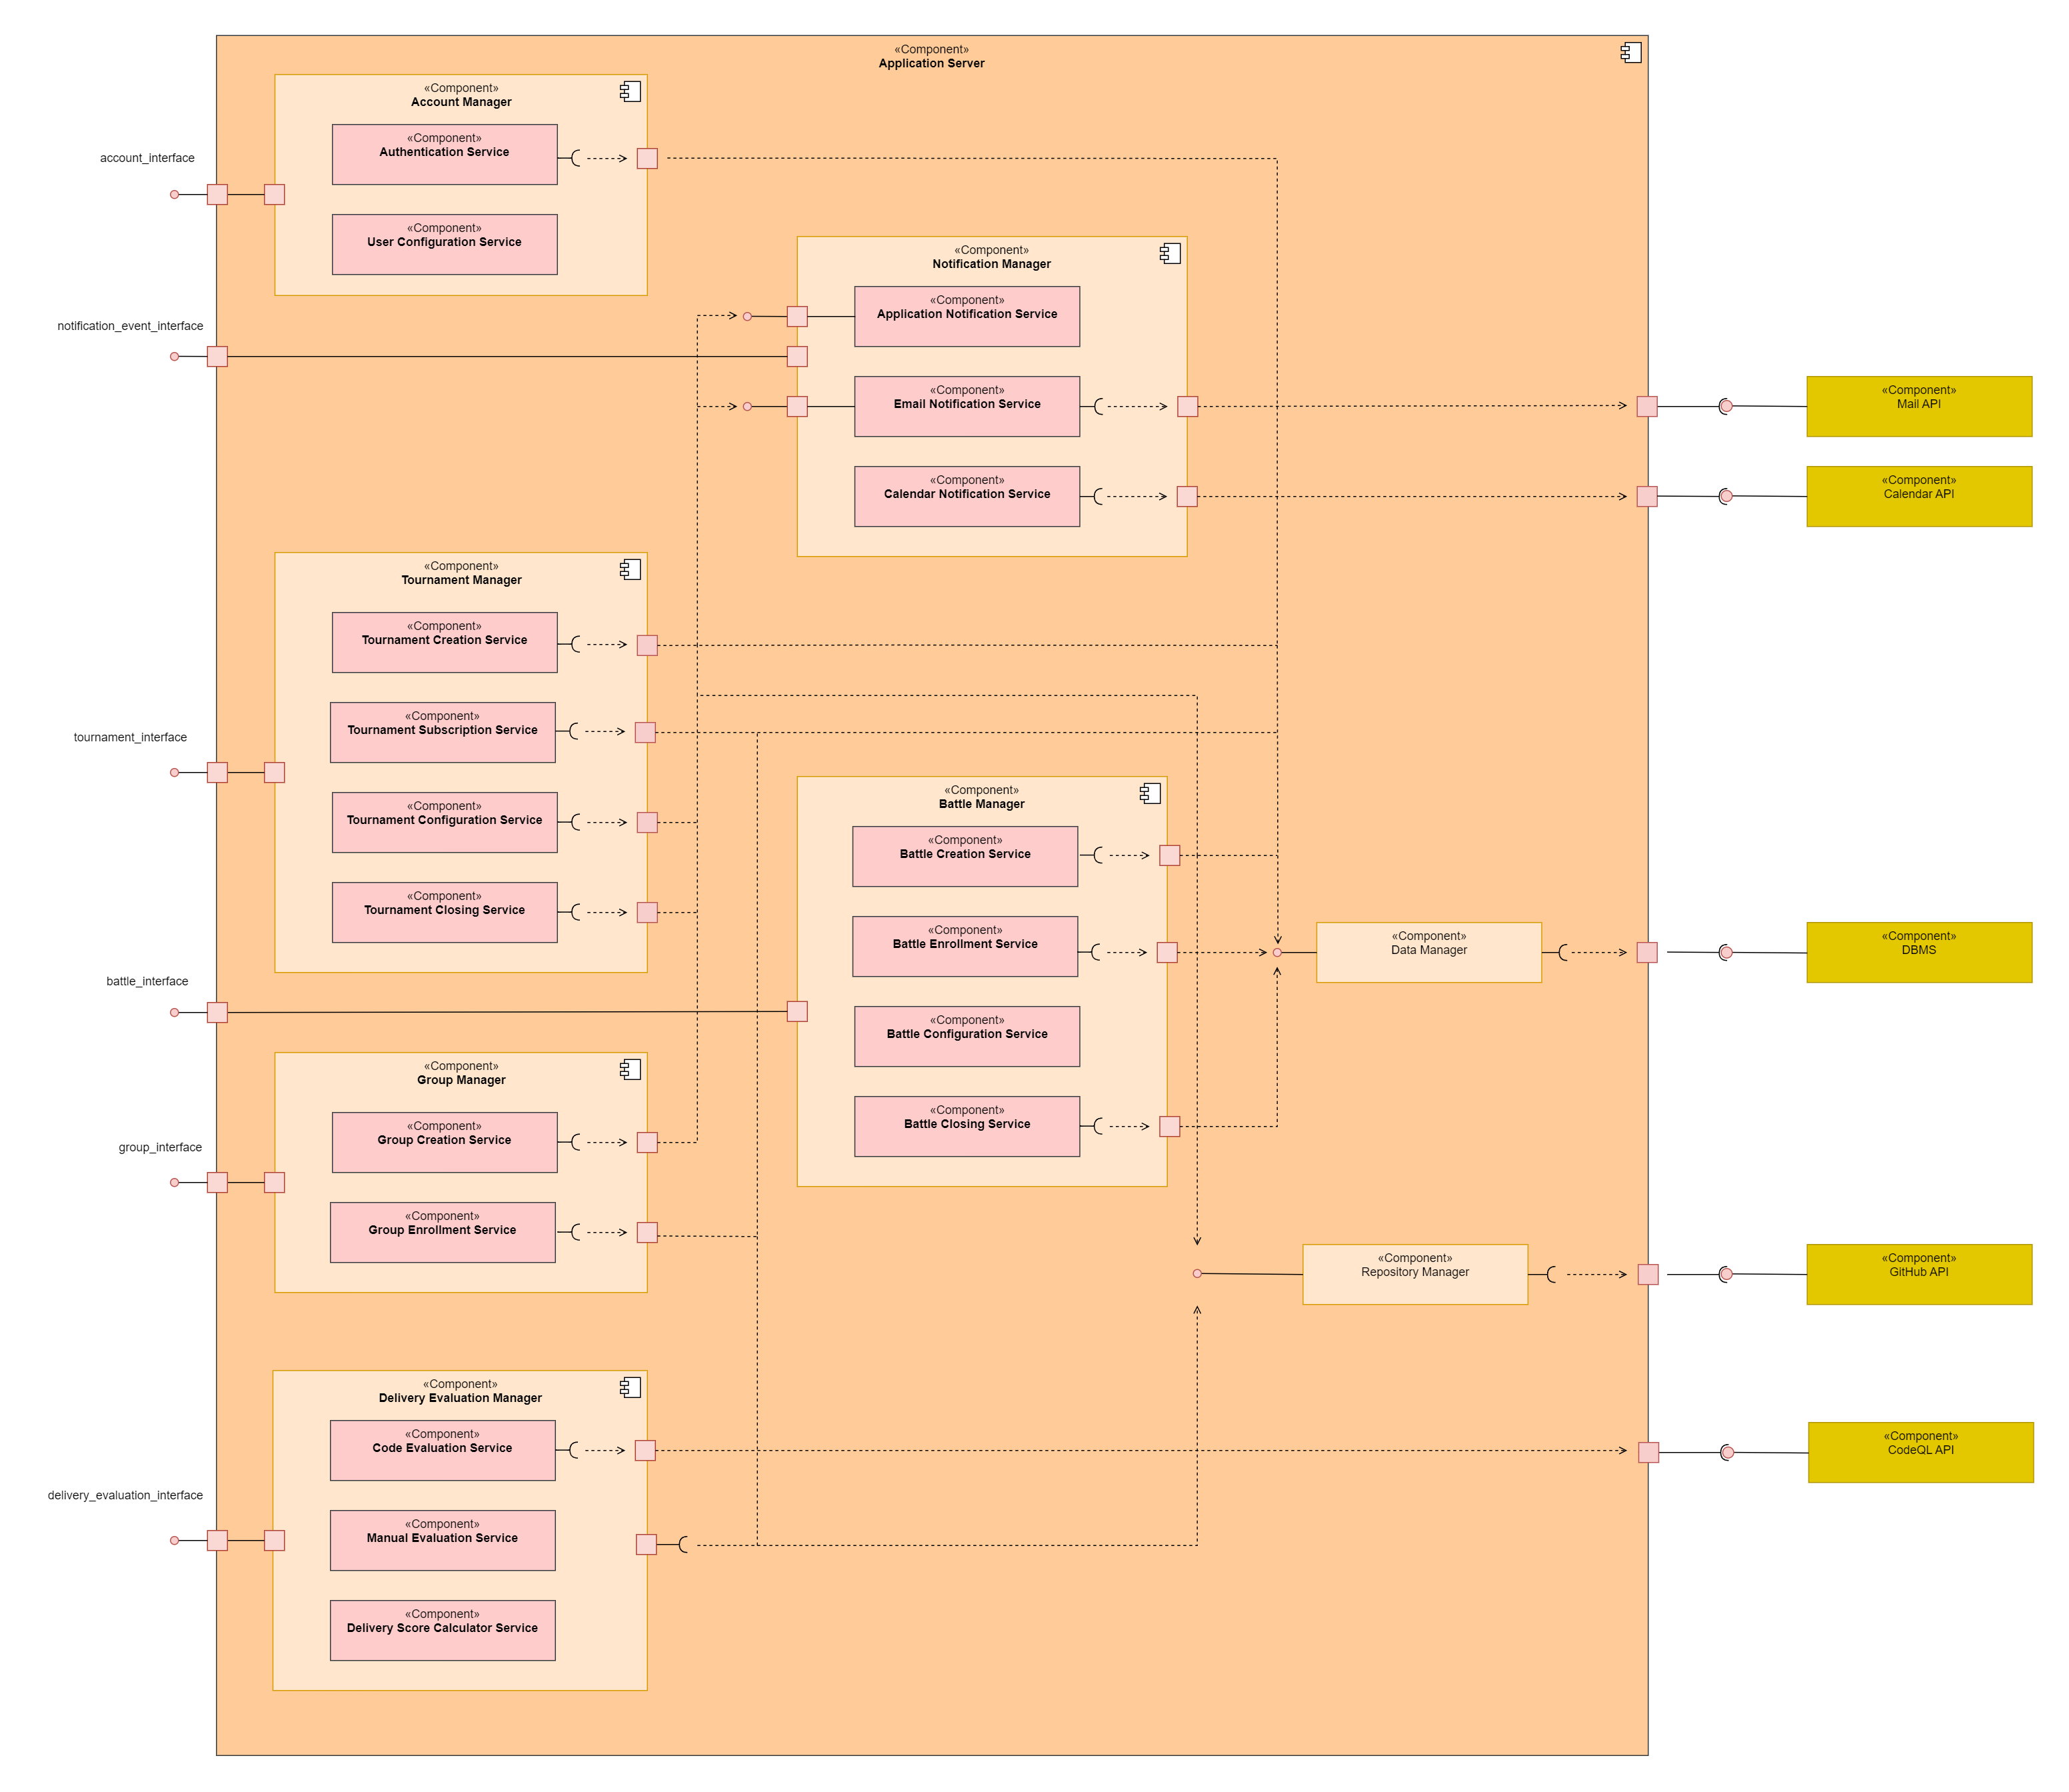
\includegraphics[width=1.45\textwidth]{../assets/section_2/ApplicationServerComponentDiagram.png}
        \end{figure}
    \newpage
    \restoregeometry
    The previous component diagram provides a detailed view of the Application Server, showing its internal structure and the interactions between its components. Since such diagram is focused on the internal structure of the server, external elements are represented in a simplified way.\\
    Description of each component:
    \begin{itemize}
        \item \textbf{Account Manager:} manages all the account related functionalities, like the authentication process and the setting of user's information.
        \begin{itemize}
            \item \textbf{Authentication Service:} handles all the functionalities related to the authentication of the user (log in, log out, sign up), after the user has authenticated through this service, he/she can use the application
            \item \textbf{User Configuration Service:} it handles the operations related to getting and setting user-configurable properties like its nickname and phone number
        \end{itemize}
        \item \textbf{Tournament Manager:} it manages all the functions related to the set-up, management and closure of a tournament
        \begin{itemize}
            \item \textbf{Tournament Creation Service:} it handles the creation of a new tournament by Educator, also checking in the database if another tournament with the same name does already exist
            \item \textbf{Tournament Subscription Service:} handles the operations required when a user requests to subscribe to a certain tournament, like adding his/her name to the list of subscribed users in the database
            \item \textbf{Tournament Configuration Service:} allows the modification of some Tournament properties, like its name, description or main picture
            \item \textbf{Tournament Closing Service:} allows to perform the operations required whenever an educator requires to close a tournament, including the check whether there is still an ongoing battle
        \end{itemize}
        \item \textbf{Battle Manager:} is responsible for all the functionalities related to code battles in the application
        \begin{itemize}
            \item \textbf{Battle Creation Service:} it allows to perform the operations required whenever a new battle is created by an educator, like uploading the corresponding CodeKata and setting the constraints required for each group to join
            \item \textbf{Battle Enrollment Service:} it handles the required operations and checks that the system has to make whenever a user wants to enroll into a battle
            \item \textbf{Battle Configuration Service:} allows getting and modifying battle-related properties, like its title, or description
            \item \textbf{Battle Closing Service:} it handles all the operations required when a battle is closed ahead of time, like the set-up of a message explaining the motivation of such closure
        \end{itemize}
        \item \textbf{Group Manager:} manages all the functionalities related to groups, like the authentication process and the setting of user's information.
        \begin{itemize}
            \item \textbf{Group Creation Service:} handles the creation of a new group by a student, including the required checks on whether he/she is enrolled into the battle he/she wants to create a group for and if that group name is already in use 
            \item \textbf{Group enrollment Service:} allows the enrollment of a student into an existing group, also checking if such student is enrolled in the same battle the group has been created for
        \end{itemize}
        \item \textbf{Repository Manager:} manages the communications from and to the online repository system (GitHub), creating the repository as described by the educator, uploading the corresponding CodeKata. When the battle is started it also automatically pulls every user's push of a new solution and sends it to the Delivery Evaluation Manager
        \item \textbf{Delivery Evaluation Manager:} manages the whole process of evaluation of a student's delivery, starting from the automated ones (according to what has been set up at creation of the battle), to the potential manual evaluation by the educator. Lastly if such manual evaluation is performed, it computes the final delivery score (battle score) according to the composition of both these evaluations
        \begin{itemize}
            \item \textbf{Code Evaluation Service:} performs all the automated evaluations that have been set up at battle-creation time, including the static analysis of the quality level of the sources through external APIs (CodeQL)
            \item \textbf{Manual Evaluation Service:} if a manual evaluation has been set up to be performed after the automated ones at battle-creation time, this component allows the educator to manually assign an evaluation to each student delivery
            \item \textbf{Delivery Score Calculator Service:} this component allows for the composition of both the scores given by the automated evaluation and the one given manually by the educator, by adding or subtracting the score manually assigned by the educator to the one that has been automatically given, this service has also been introduced in order to allow in the future for the possible inclusion of new ways to perform this composition (like a weighted average or by allowing the educator to increase/decrease the automated score assigned for a specific aspect of the code)
        \end{itemize}
        \item \textbf{Notification Event Manager:} controls the different kind of way in which a notification can be sent to the user
        \begin{itemize}
            \item \textbf{Application Notification Service:} handles the in-application notifications, so the ones that will remain only in the application itself, and shown through a specific icon on the user's dashboard
            \item \textbf{Email Notification Service:} handles those notifications that will also be sent as an email to the user, to highlight their greater importance
            \item \textbf{Calendar Notification Service:} handles a special type of notification occurring when a battle is created in a tournament to which the student is subscribed that will also create (if such permission has been given by the user) an event in the user's Google Calendar application for the corresponding date and time
        \end{itemize}
        \item \textbf{Data Manager:} this component manages the access of the application to the database representing its data layer, performing eventual pre-processing on the data if required
    \end{itemize}
    \newpage

    \subsection{Deployment View}\label{subsec:deployment_view}
    The deployment diagram depicted here below illustrates the distribution of different components of the web application across the network. 
    This includes the deployment of the web server, application server, and database server.
    \begin{figure}[H]
        \centering
        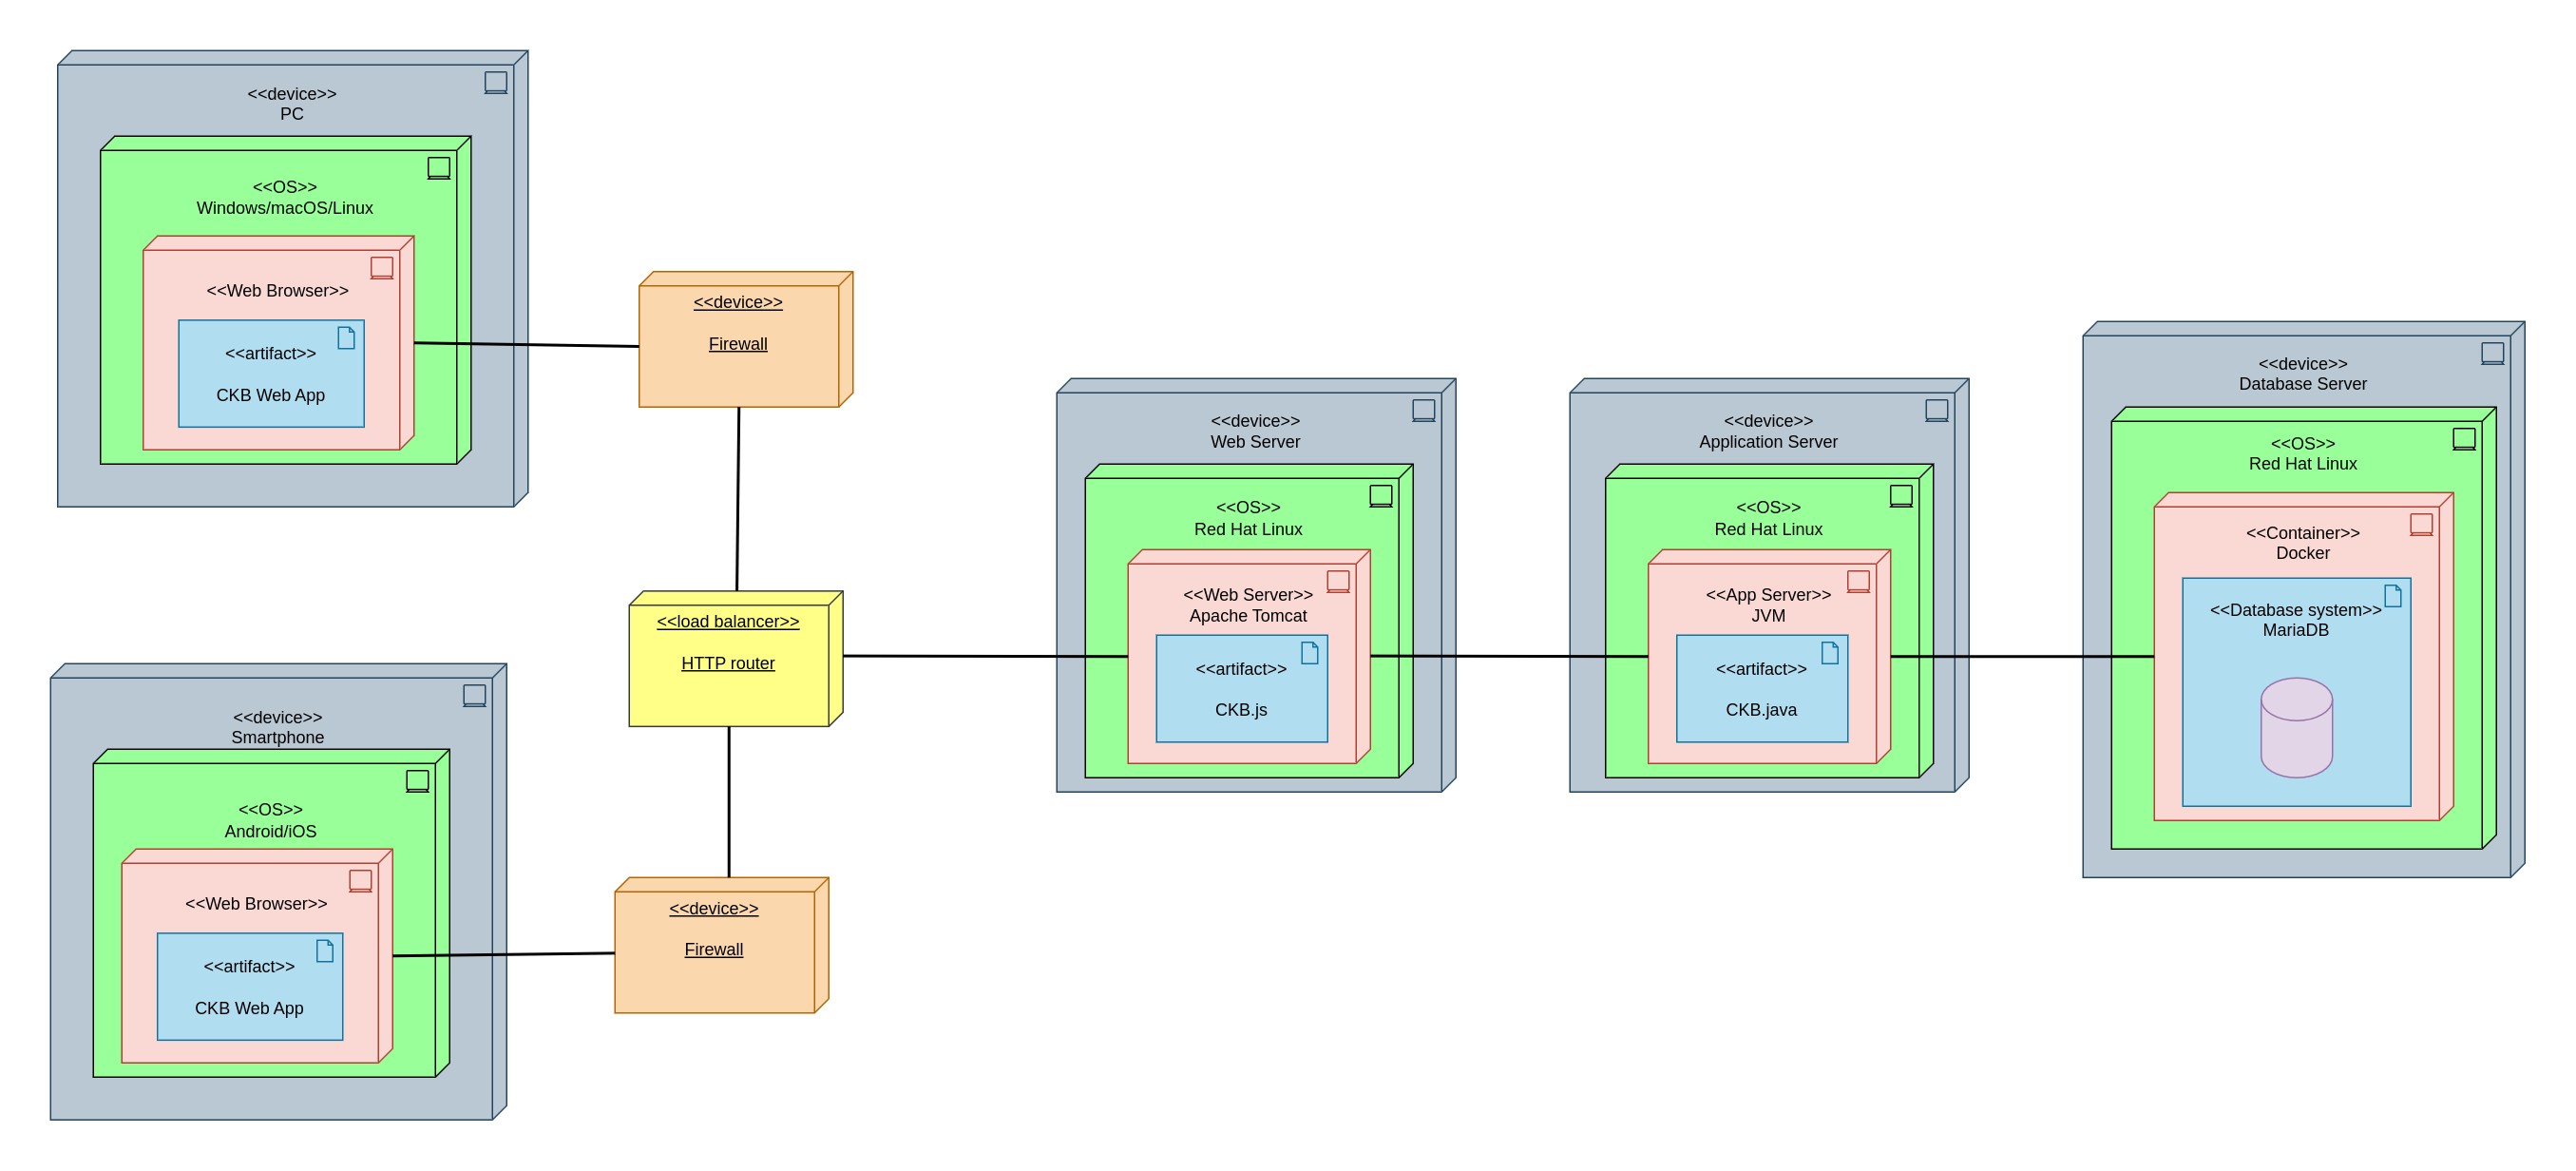
\includegraphics[width=\textwidth]{../assets/section_2/deployment_diagram.png}
        \caption{Deployment Diagram}
        \label{fig:deployment_diagram}
    \end{figure} 
    The diagram visually represents the relationships and the flow of data among these components.
    \begin{itemize}
        \item {\textbf{Smartphone/PC}: the user's device is used for displaying the web application. It's utilized to access and interact with the web application through the web browser and the HTTPS protocol.}
        \item {\textbf{Firewall}: fundamental security device, safeguards the network against unauthorized access by filtering both incoming and outgoing traffic.
        A proper configuration of the firewall is essential to ensure the security of the system.}
        \item {\textbf{Load Balancer}: it serves to evenly distribute incoming web traffic among multiple servers, ensuring the continuous availability of the web application and enhancing the system's scalability.}
        \item {\textbf{Web Server}: it's the server in charge of handling the HTTPS requests coming from the clients.
        It handles the communication between the clients and the platform itself.}
        \item {\textbf{Application Server}: responsible for the business logic of the system, it manages the requests coming from the web server. 
        It's also in charge of the communication with the database server.}
        \item {\textbf{Database server}: it's the server responsible for storing all the information within the web application.
        A dockerized\footnote{An application is dockerized if it runs inside a Docker container} version of MariaDB will be used as the database management system in order to further enhance flexibility and scalability. We opted for a relational DBMS, particularly MariaDB, due to its robust data integrity features, seamless scalability, and ACID compliance. Furthermore, MariaDB's open-source nature, active community support, and compatibility with MySQL make it a cost-effective and reliable choice for our database needs.}
    \end{itemize}
    \newpage

    
    \subsection{Component Interfaces}\label{subsec:component_interfaces}
    The following diagram provides a comprehensive depiction of the interfaces and their associated methods offered by each component within the CKB platform. 
    It is essential to acknowledge that the delineated methods do not precisely mirror the final version intended for implementation; rather, they serve as a logical representation.
    \begin{figure}[h]
        \centering
        \hspace*{-3cm}
        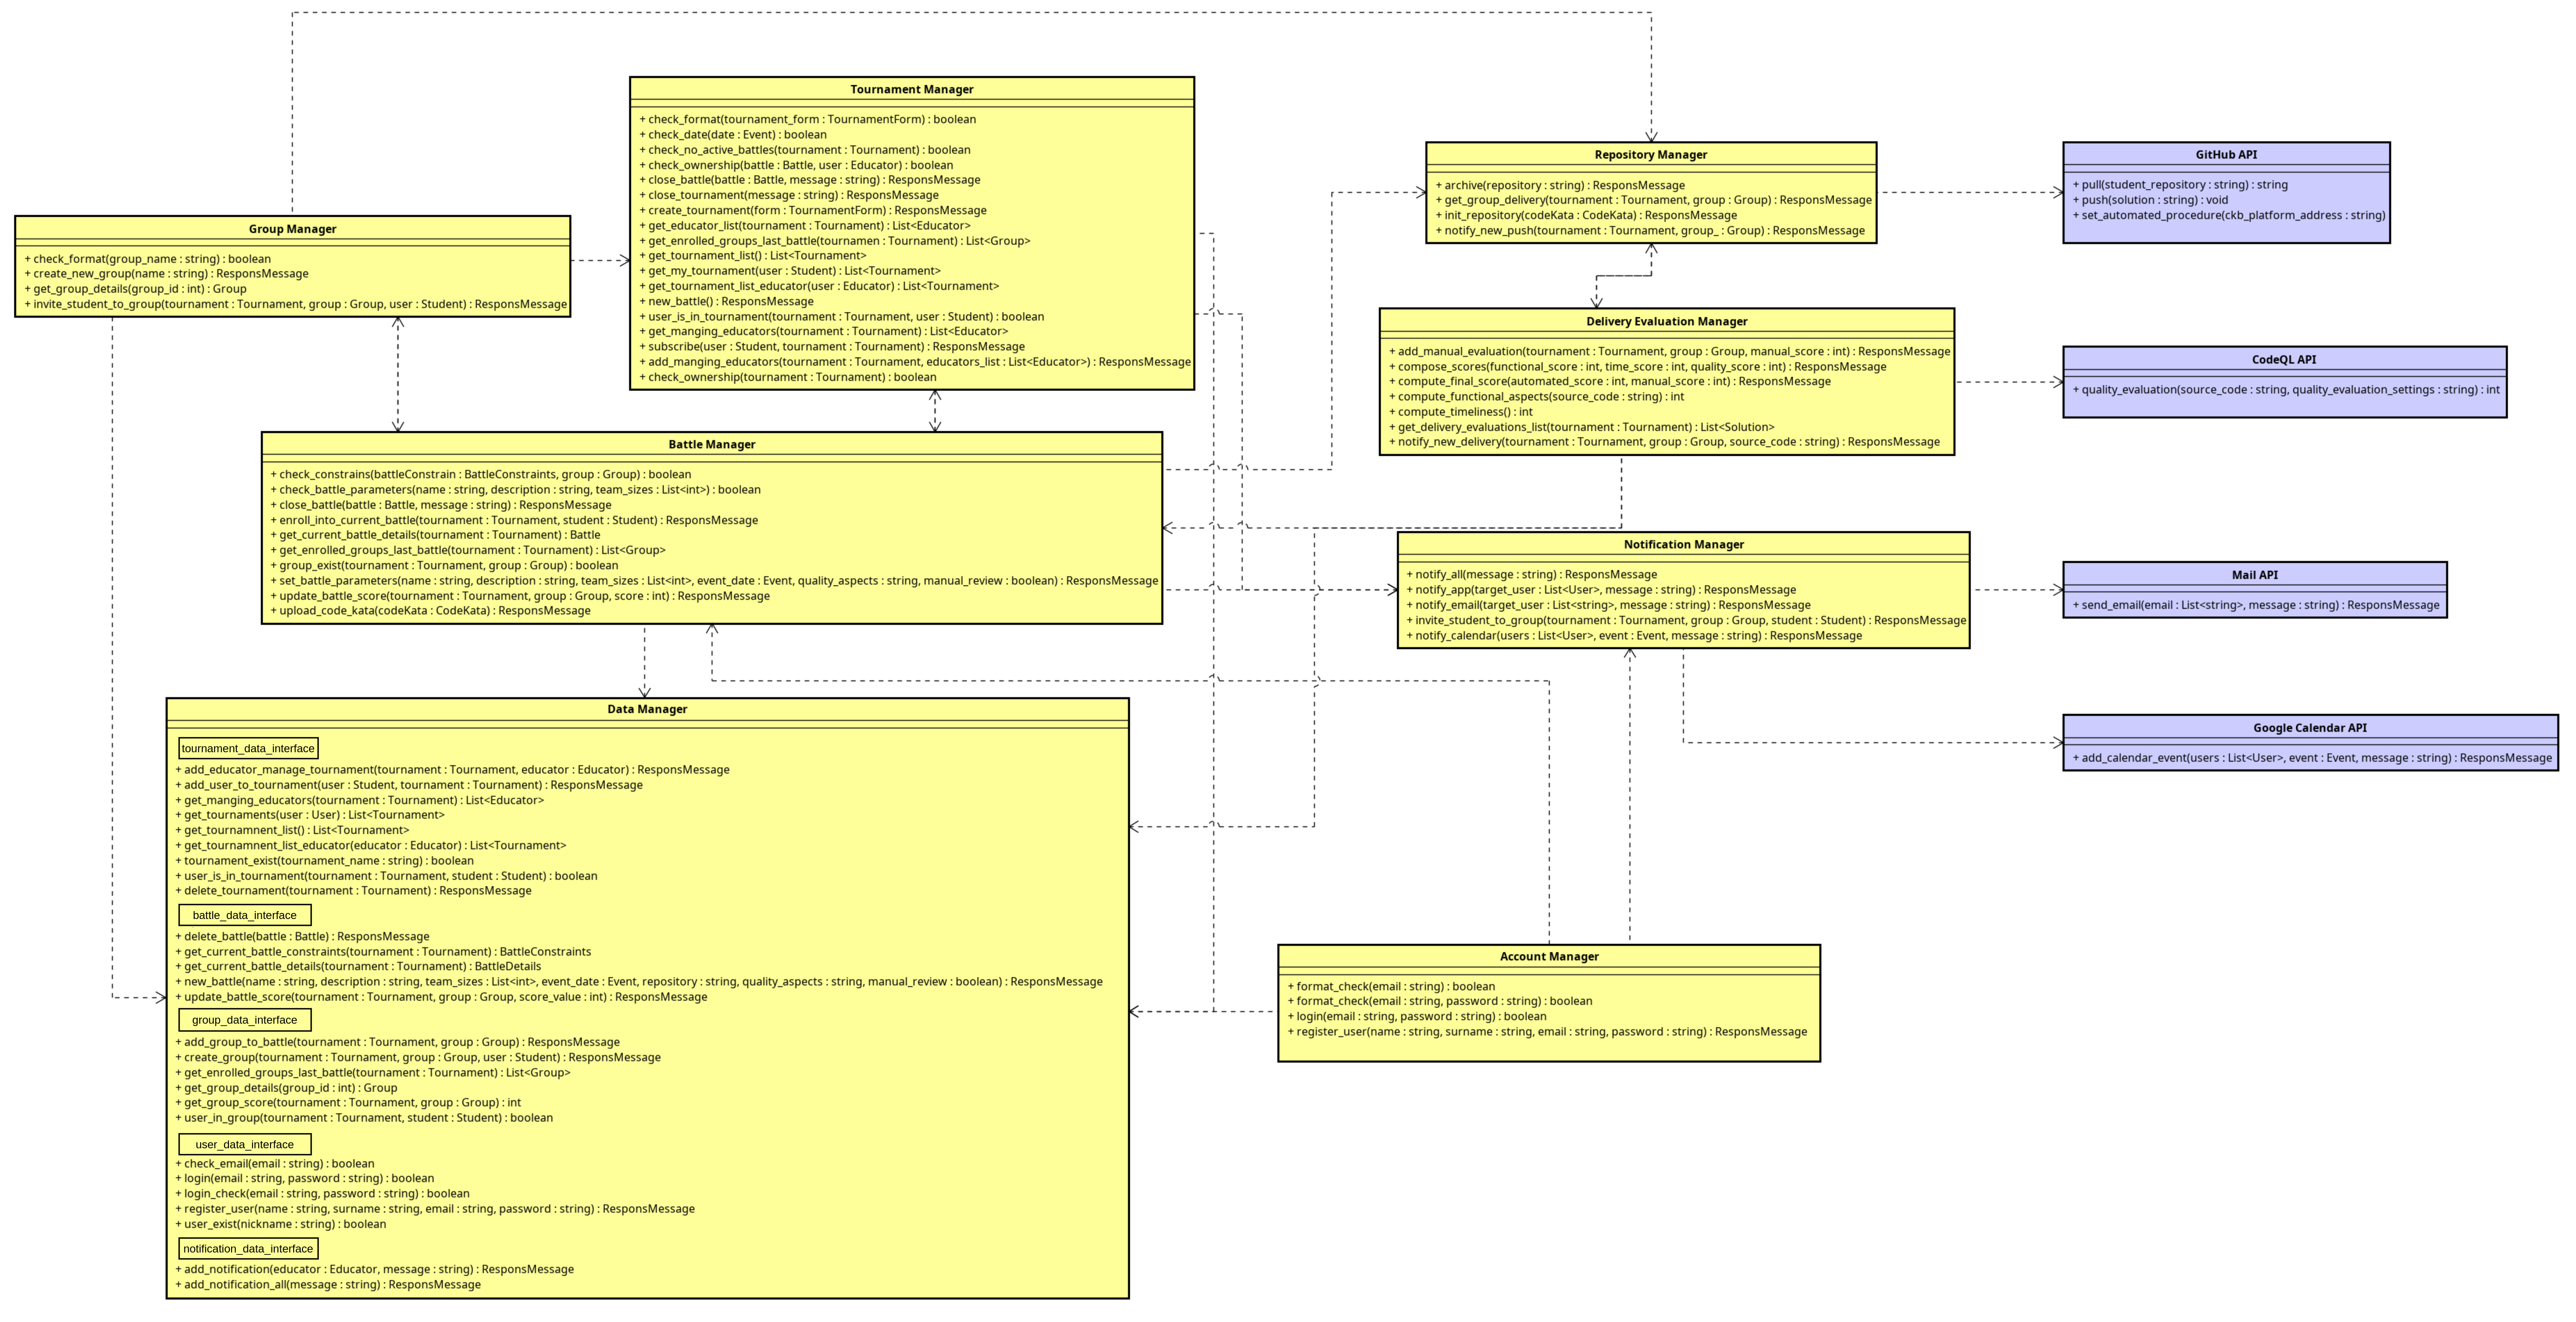
\includegraphics[width=1.4\textwidth]{../assets/section_2/interfacesDiagram.png}
        \caption{Component Interface diagram}
    \end{figure}
    \newpage

    \subsection{Runtime View}\label{subsec:runtime_view}
    In this section various practical application of the system are presented through sequence diagrams.\\
    \textbf{Sign up}\\
    \begin{figure}[H]
        \centering
        \hspace*{-3cm}
        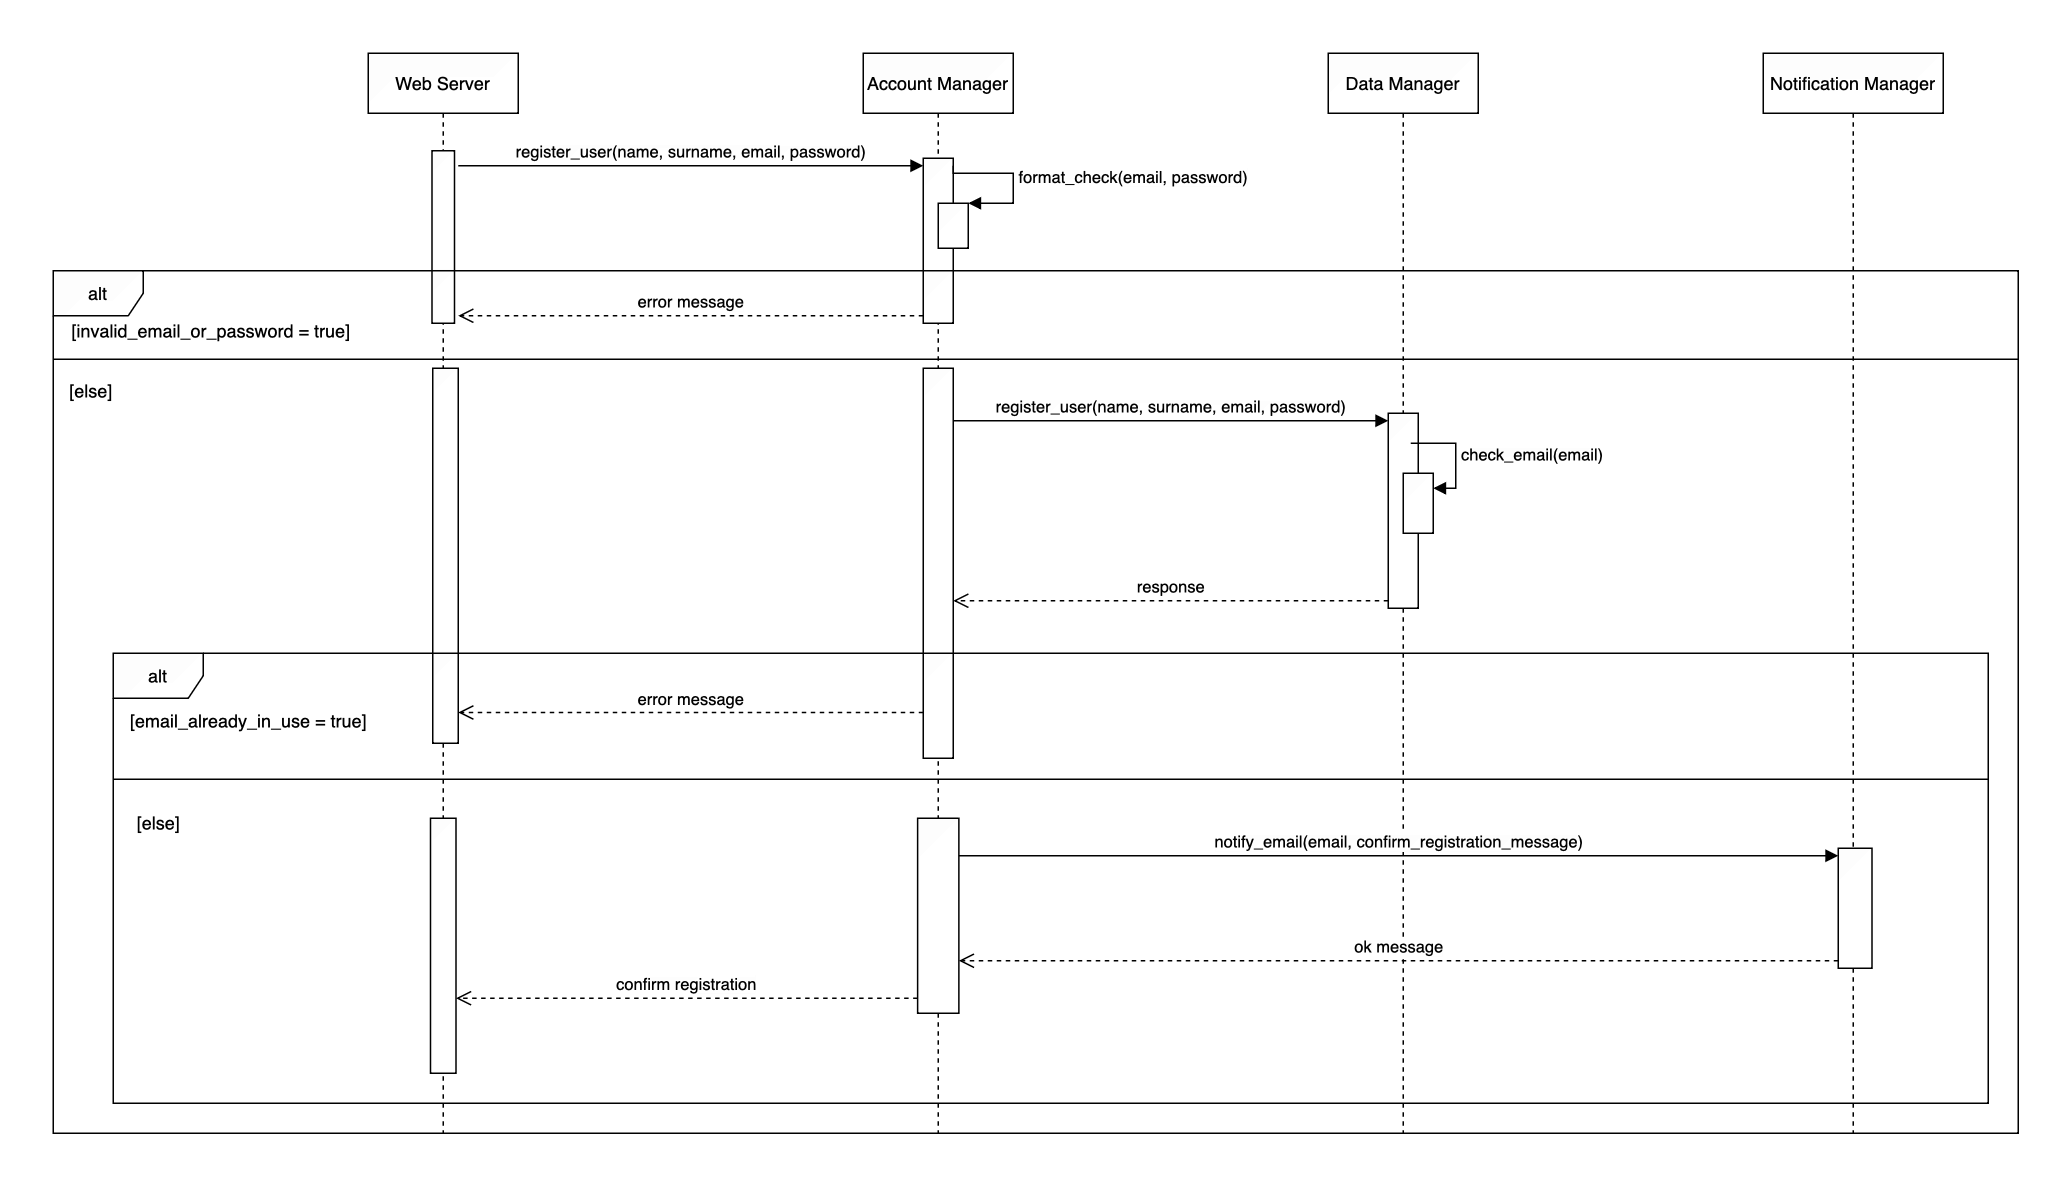
\includegraphics[width=1.35\textwidth]{../assets/section_2/SignUp.png}
    \end{figure}
    The \textit{Sign-Up} phase involves users entering their personal information into the designated fields. 
    Subsequently, the system verifies whether the email, serving as a unique identifier in the database, is already registered. 
    If the email is not found, the user is eligible to proceed with the sign-up process.
    \newpage

    \textbf{Log in}\\
    \begin{figure}[H]
        \centering
        \hspace*{-3cm}
        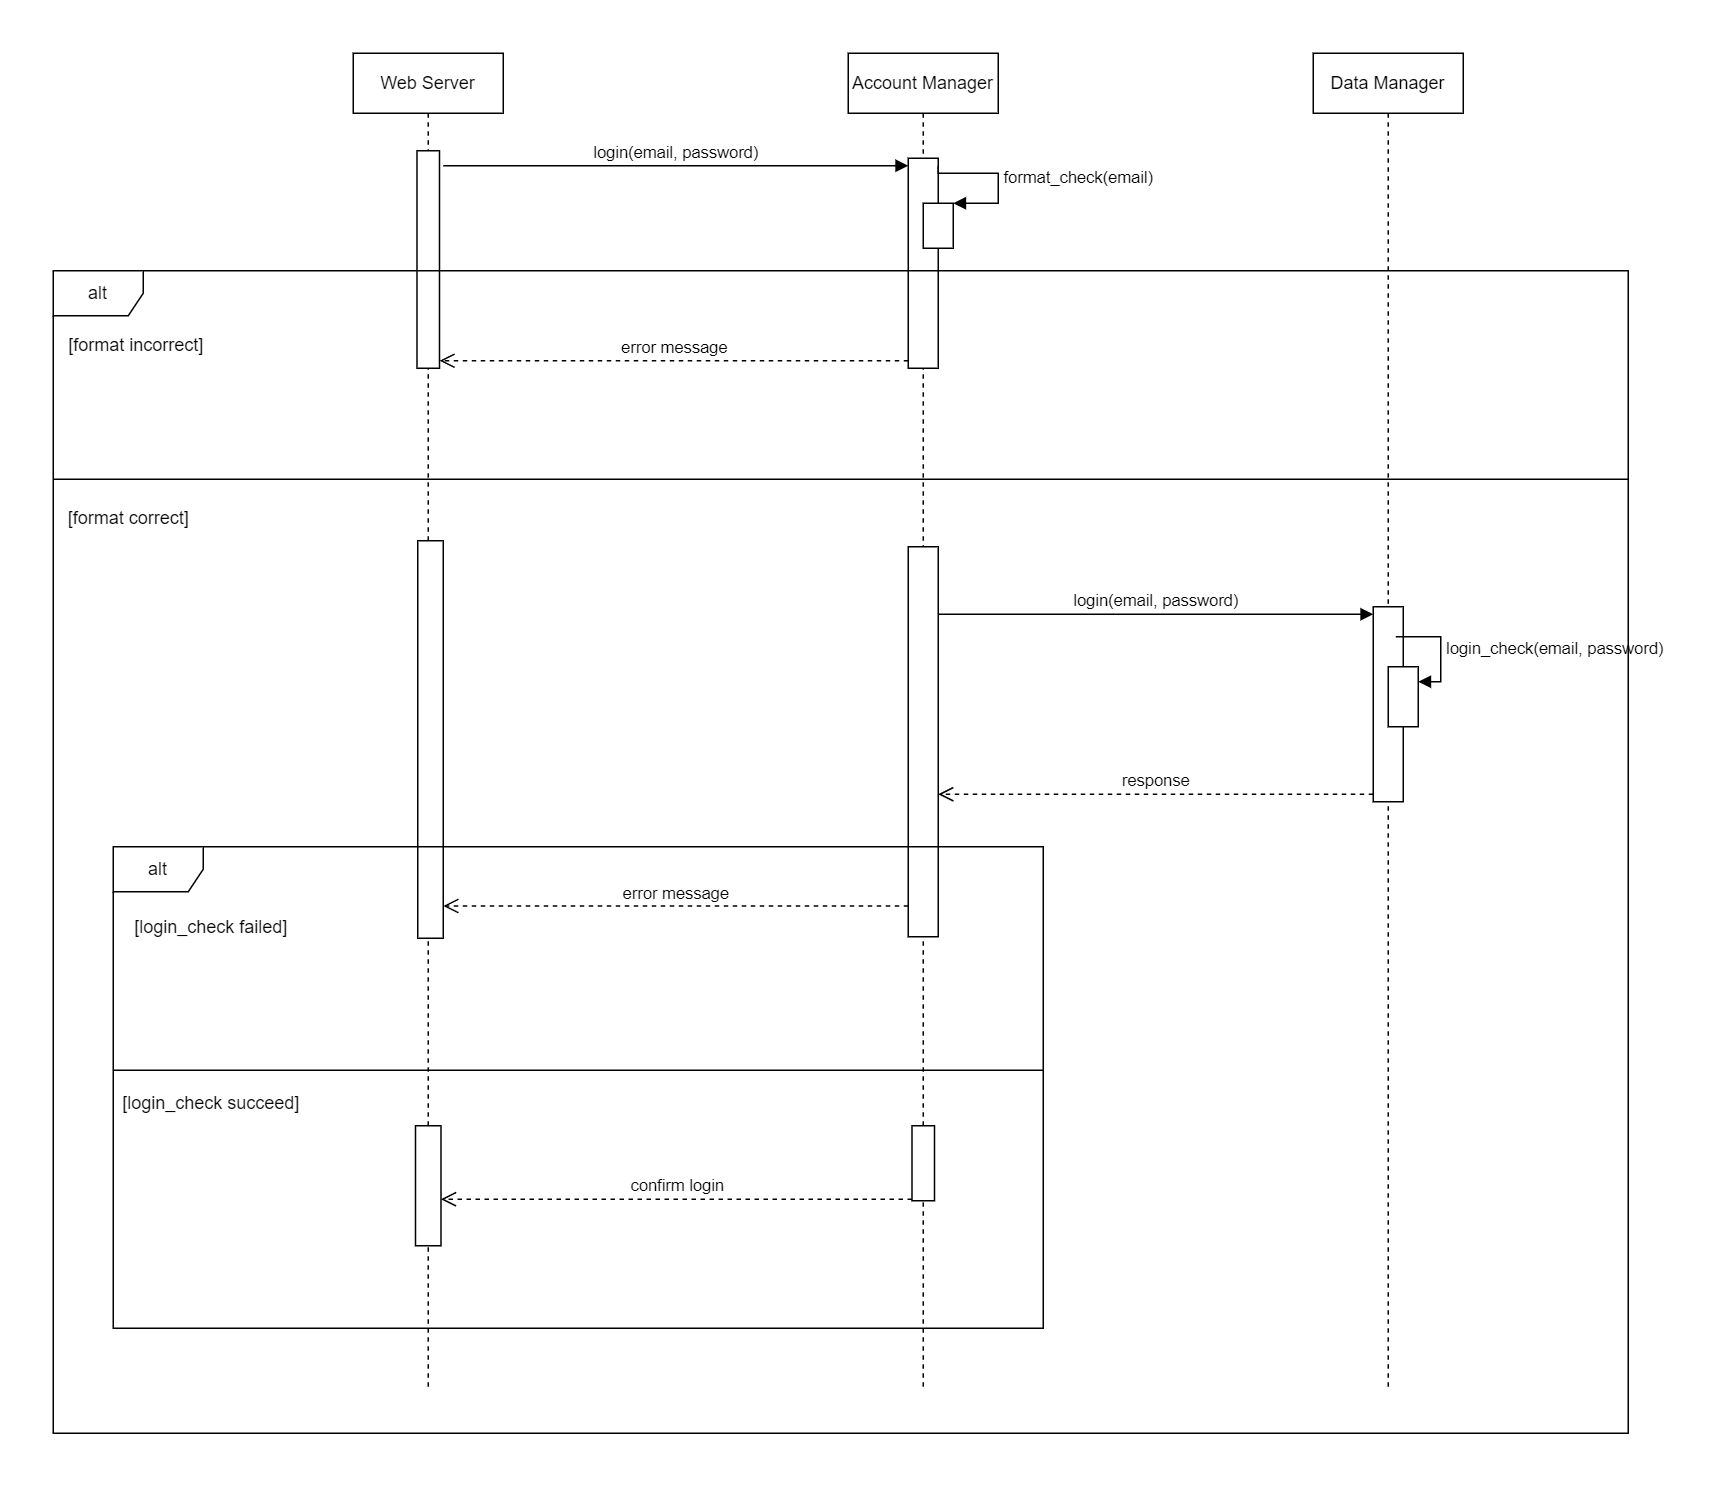
\includegraphics[width=1.35\textwidth]{../assets/section_2/login.png}
    \end{figure}
    The \textit{Log-In} phase involves users entering their credentials into the designated fields.
    Subsequently, the system verifies whether the email and password combination is valid.
    If the credentials are valid, the user is eligible to proceed with the log-in process, hence to use the CKB platform.
    \newpage

    \textbf{Create a tournament}\\
    \begin{figure}[H]
        \centering
        \hspace*{-3cm}
        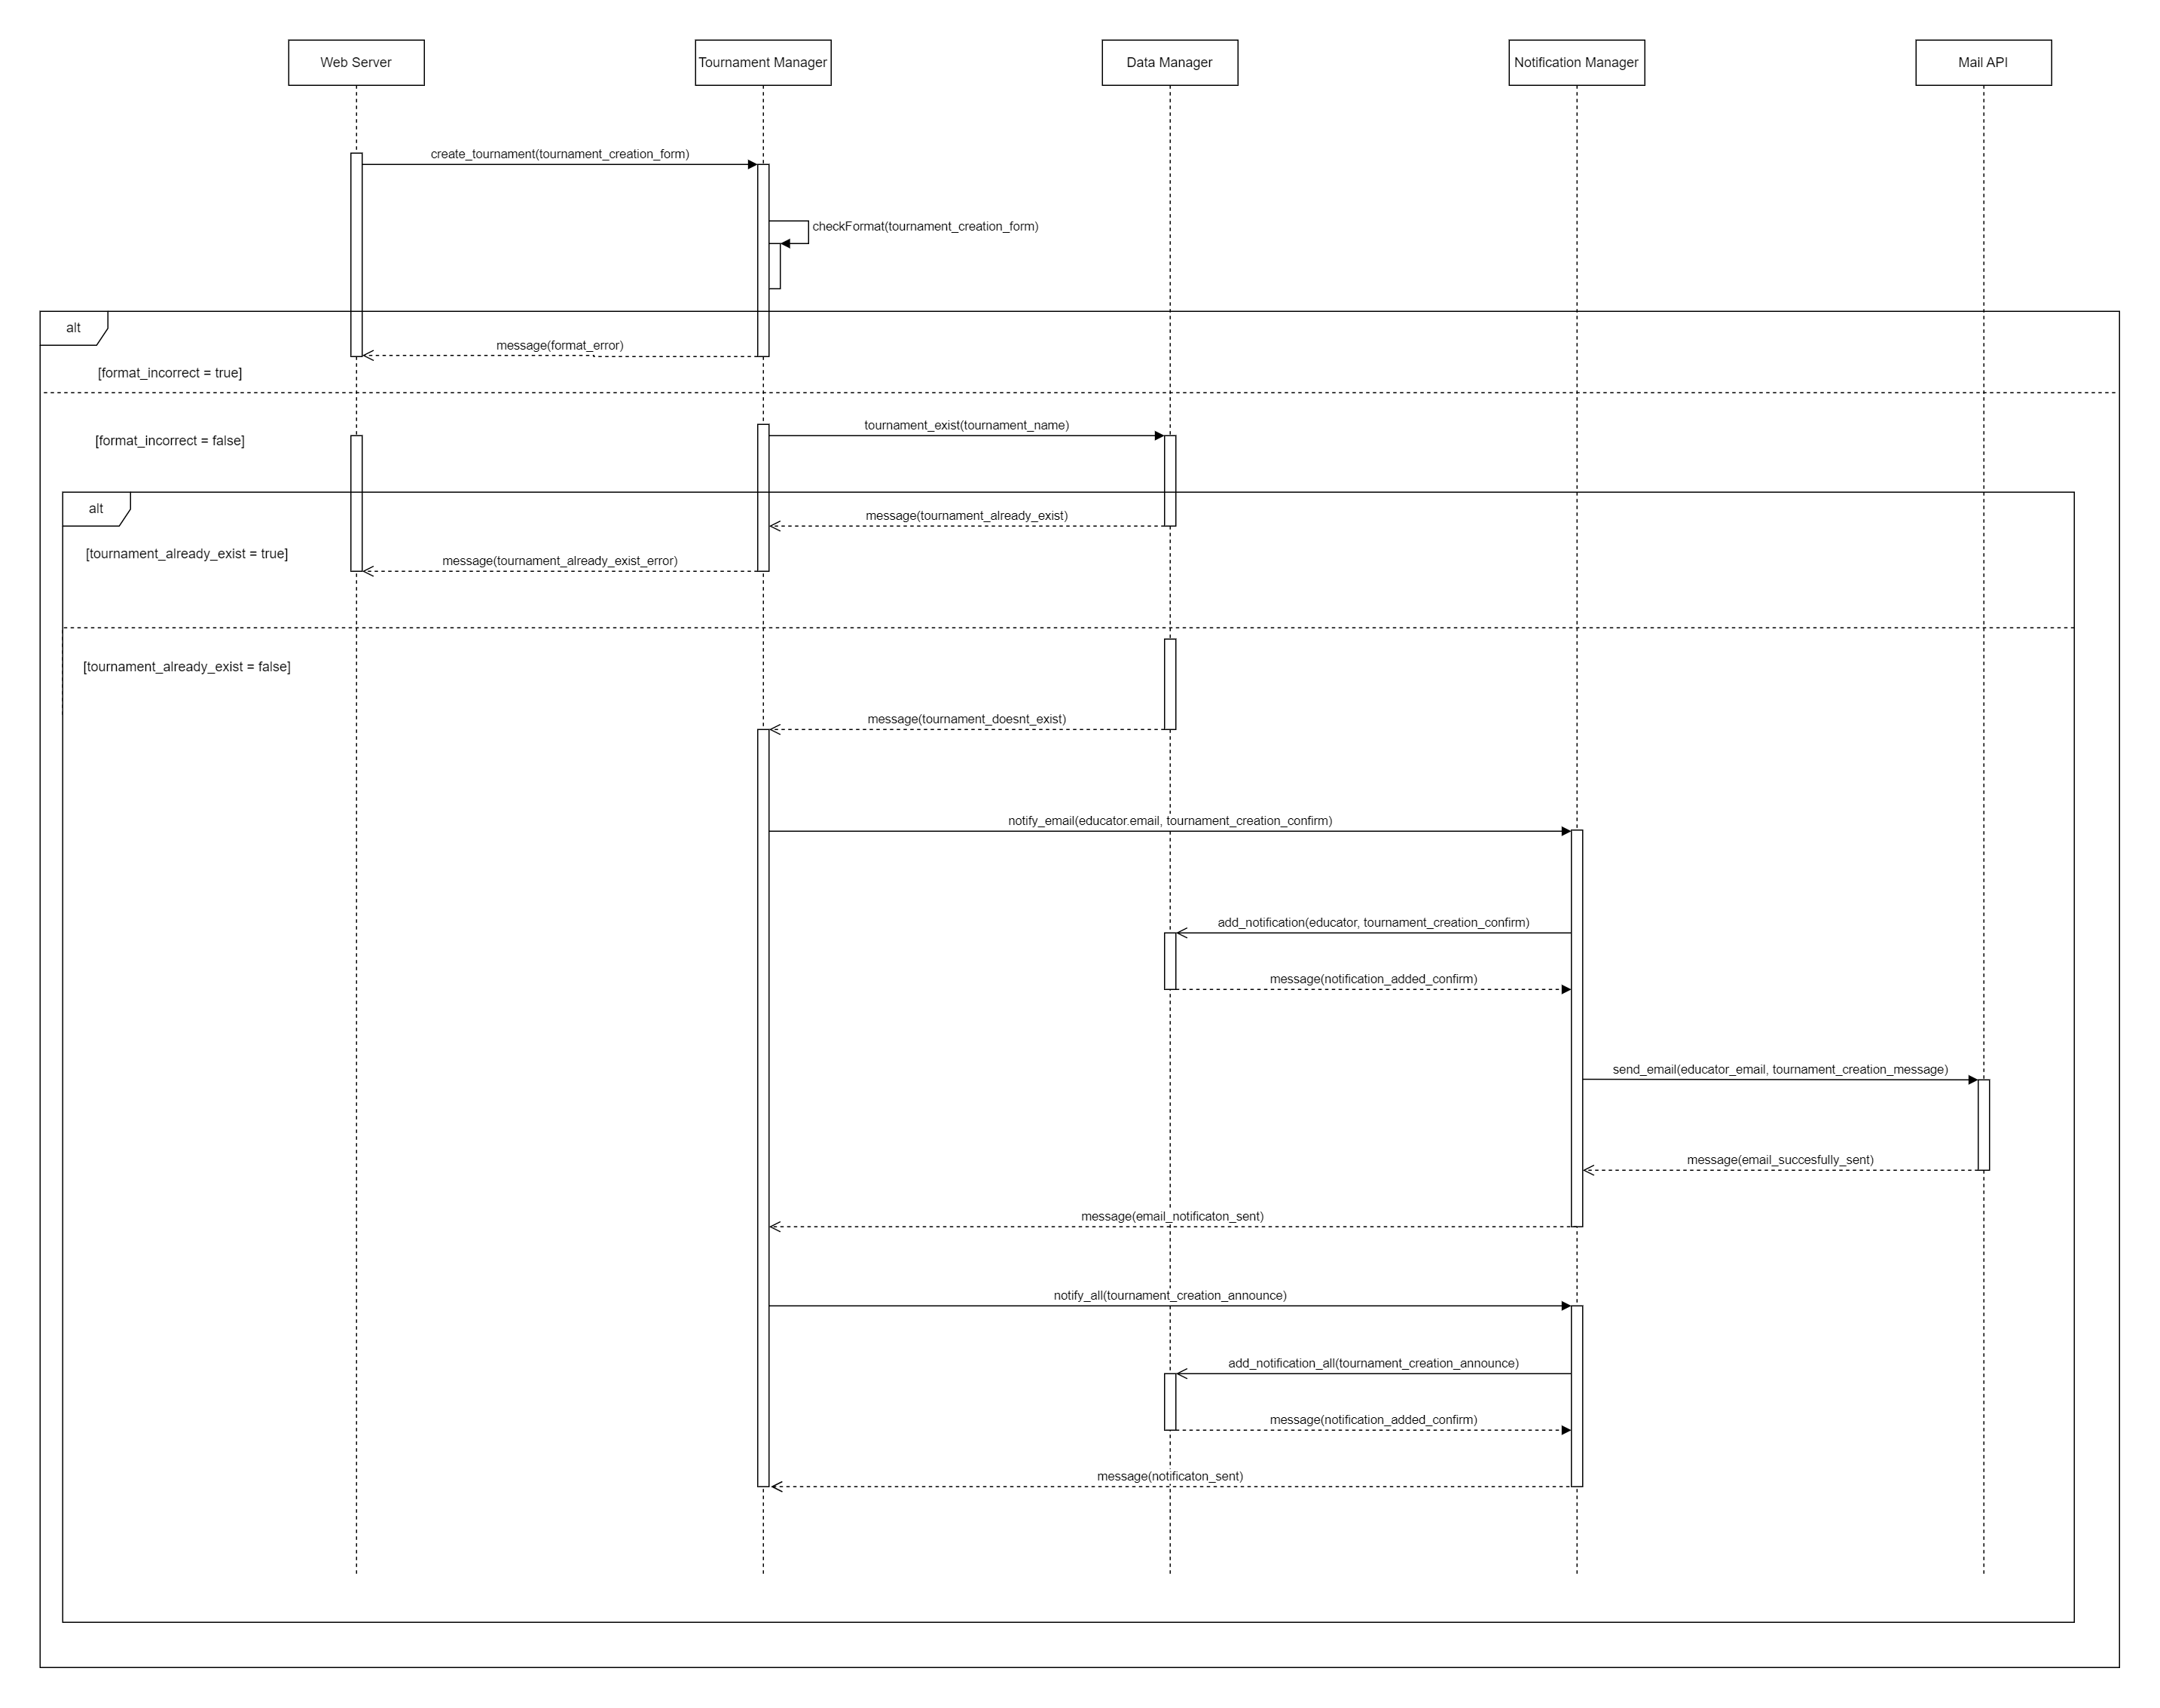
\includegraphics[width=1.35\textwidth]{../assets/section_2/CreateATournamentDiagram.png}
    \end{figure}
    The \textit{Create a tournament} phase involves an educator entering the tournament's information into the designated fields.
    In particular, after the educator has entered the tournament's name, the system verifies whether there exists another tournament with the same name.
    Upon successful verification a new tournament is created.
    A notification to all the users of the CKB platform is sent to inform them about the creation of the new tournament.
    \newpage

    \newgeometry{top = 8em}
    \textbf{Invite other educators to manage a tournament}\\
    \begin{figure}[H]
        \centering
        \hspace*{-3cm}
        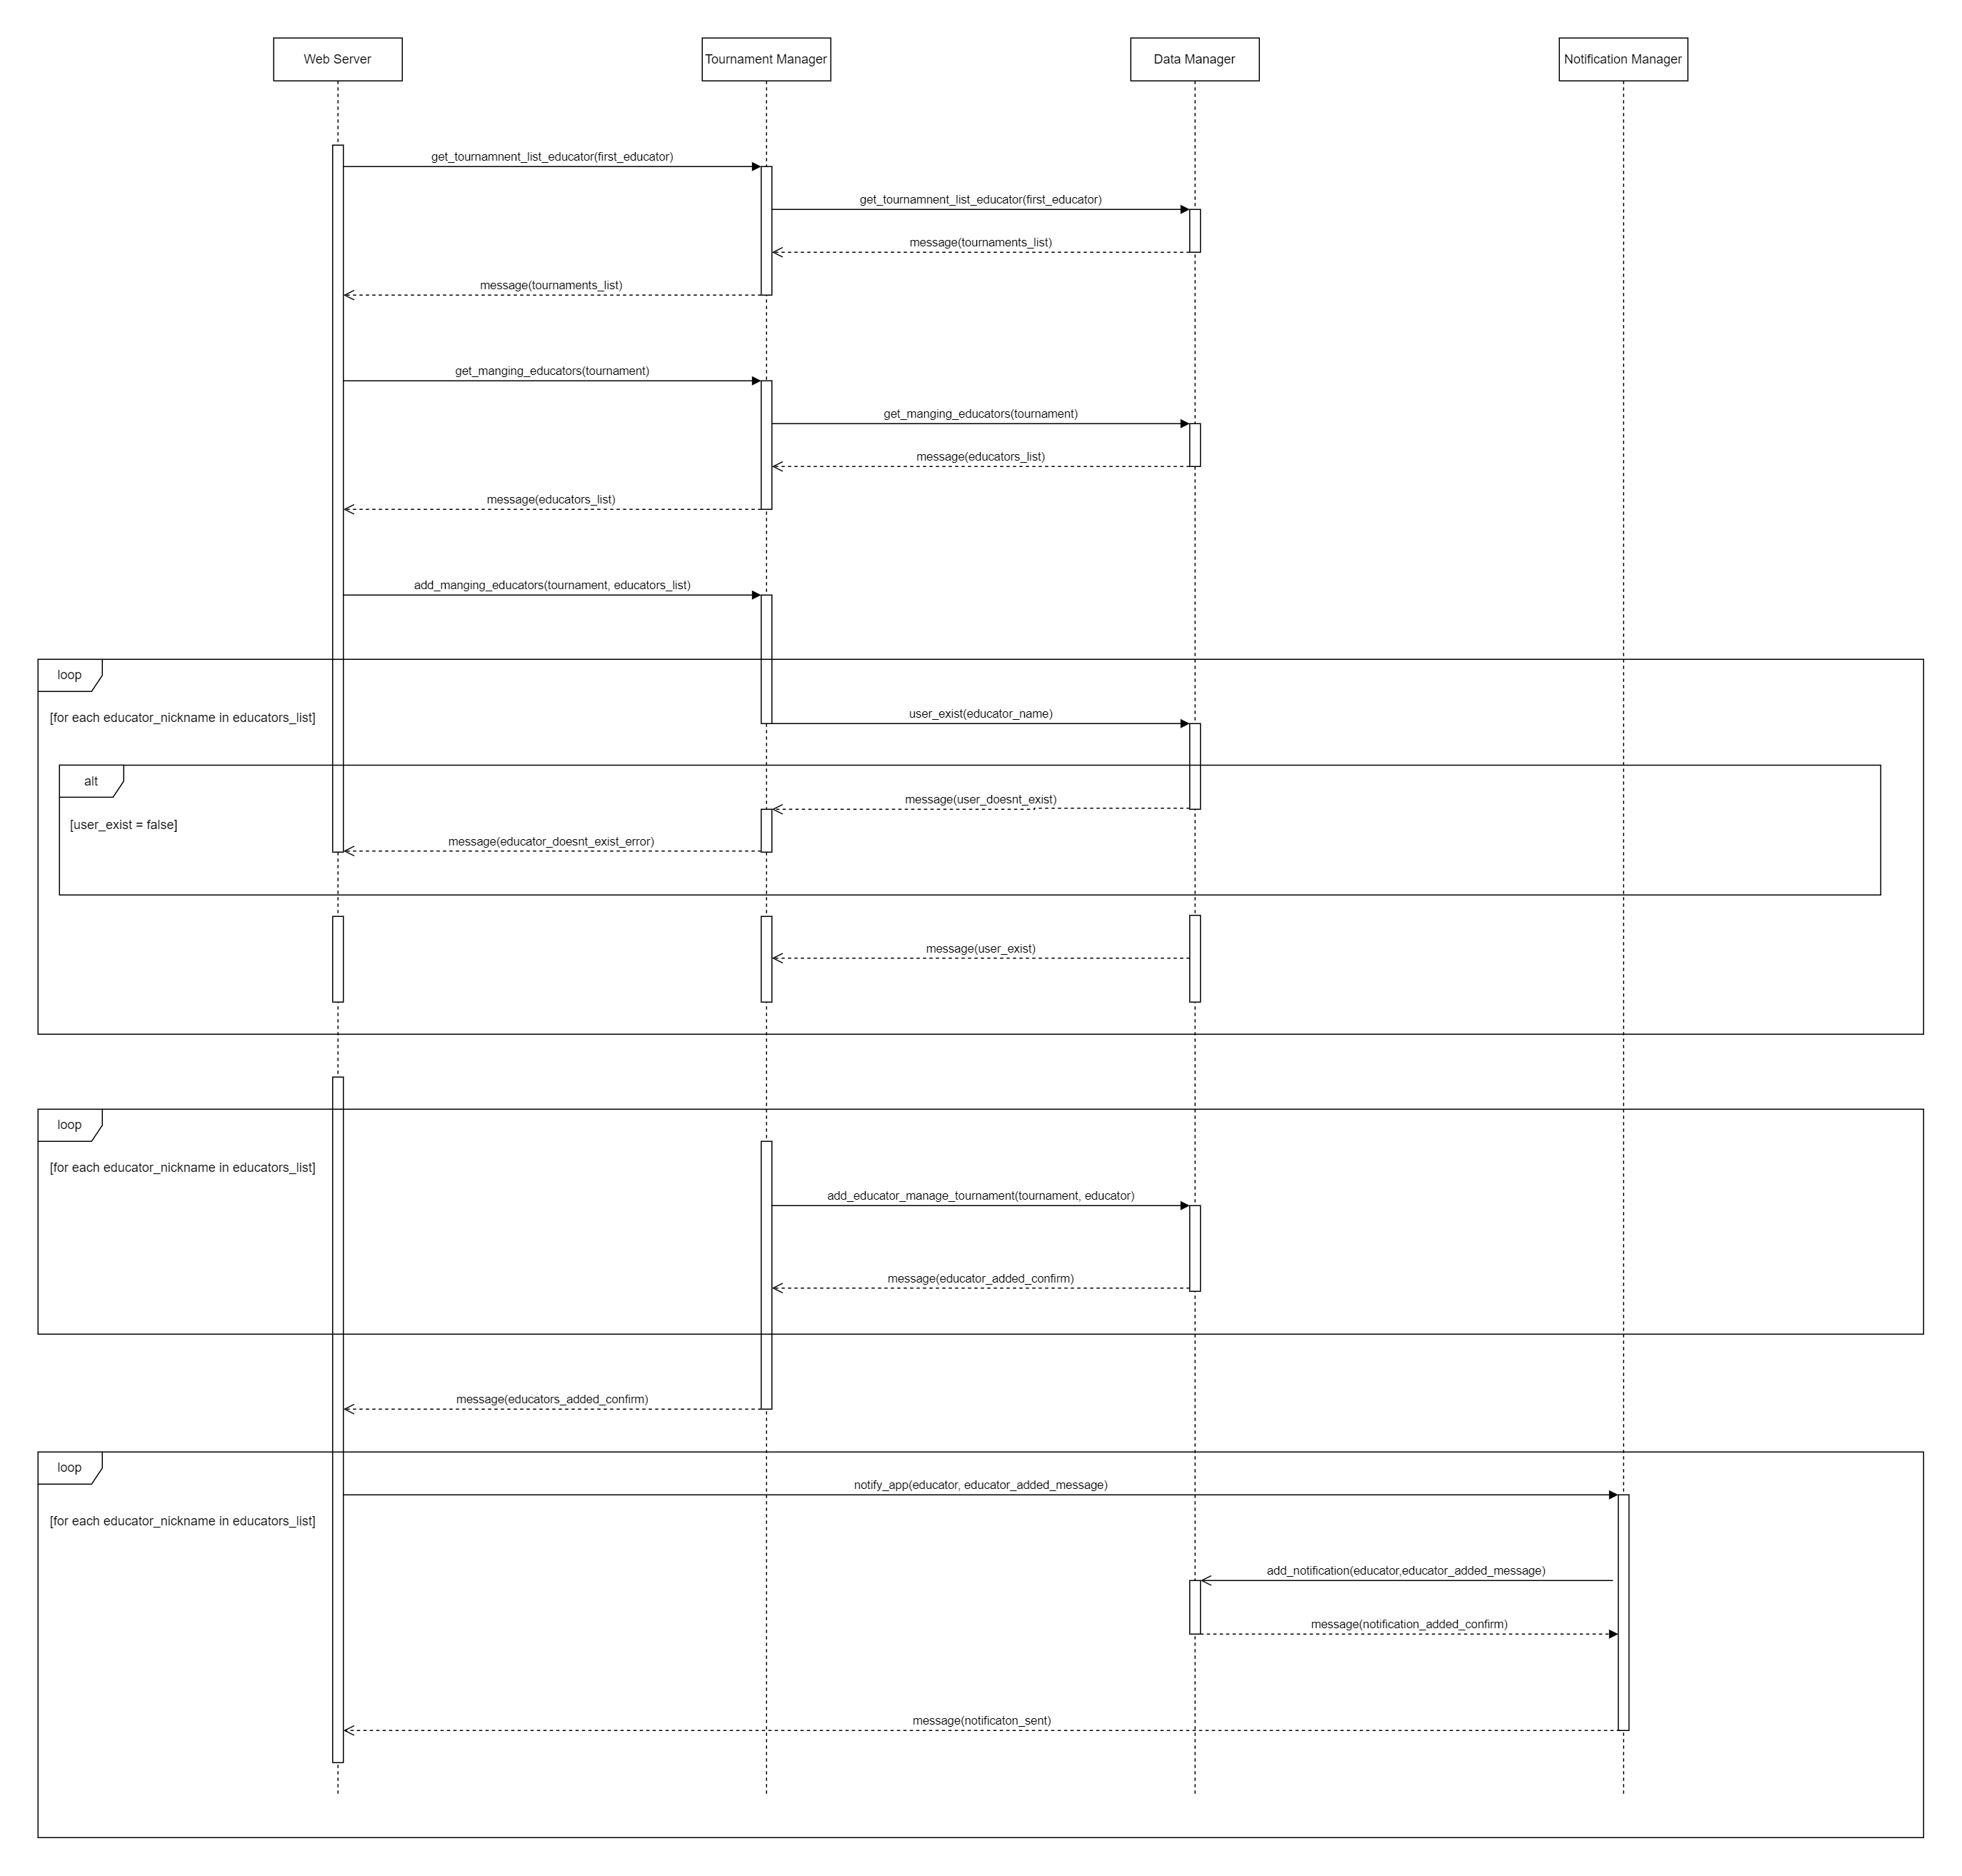
\includegraphics[width=1.35\textwidth]{../assets/section_2/InviteOtherEducatorsToManageATournament.png}
    \end{figure}
    The \textit{Invite other educators to manage a tournament} phase involves an educator entering the email of the educator he/she wants to invite into the designated field.
    Specifically, the system checks that the users exists and then sends an invitation to the educator.
    It's important to note that the educator can invite multiple educators at the same time following this procedure.
    \newpage
    \restoregeometry

    \textbf{Create a battle}
    \begin{figure}[H]
        \centering
        \hspace*{-3cm}
        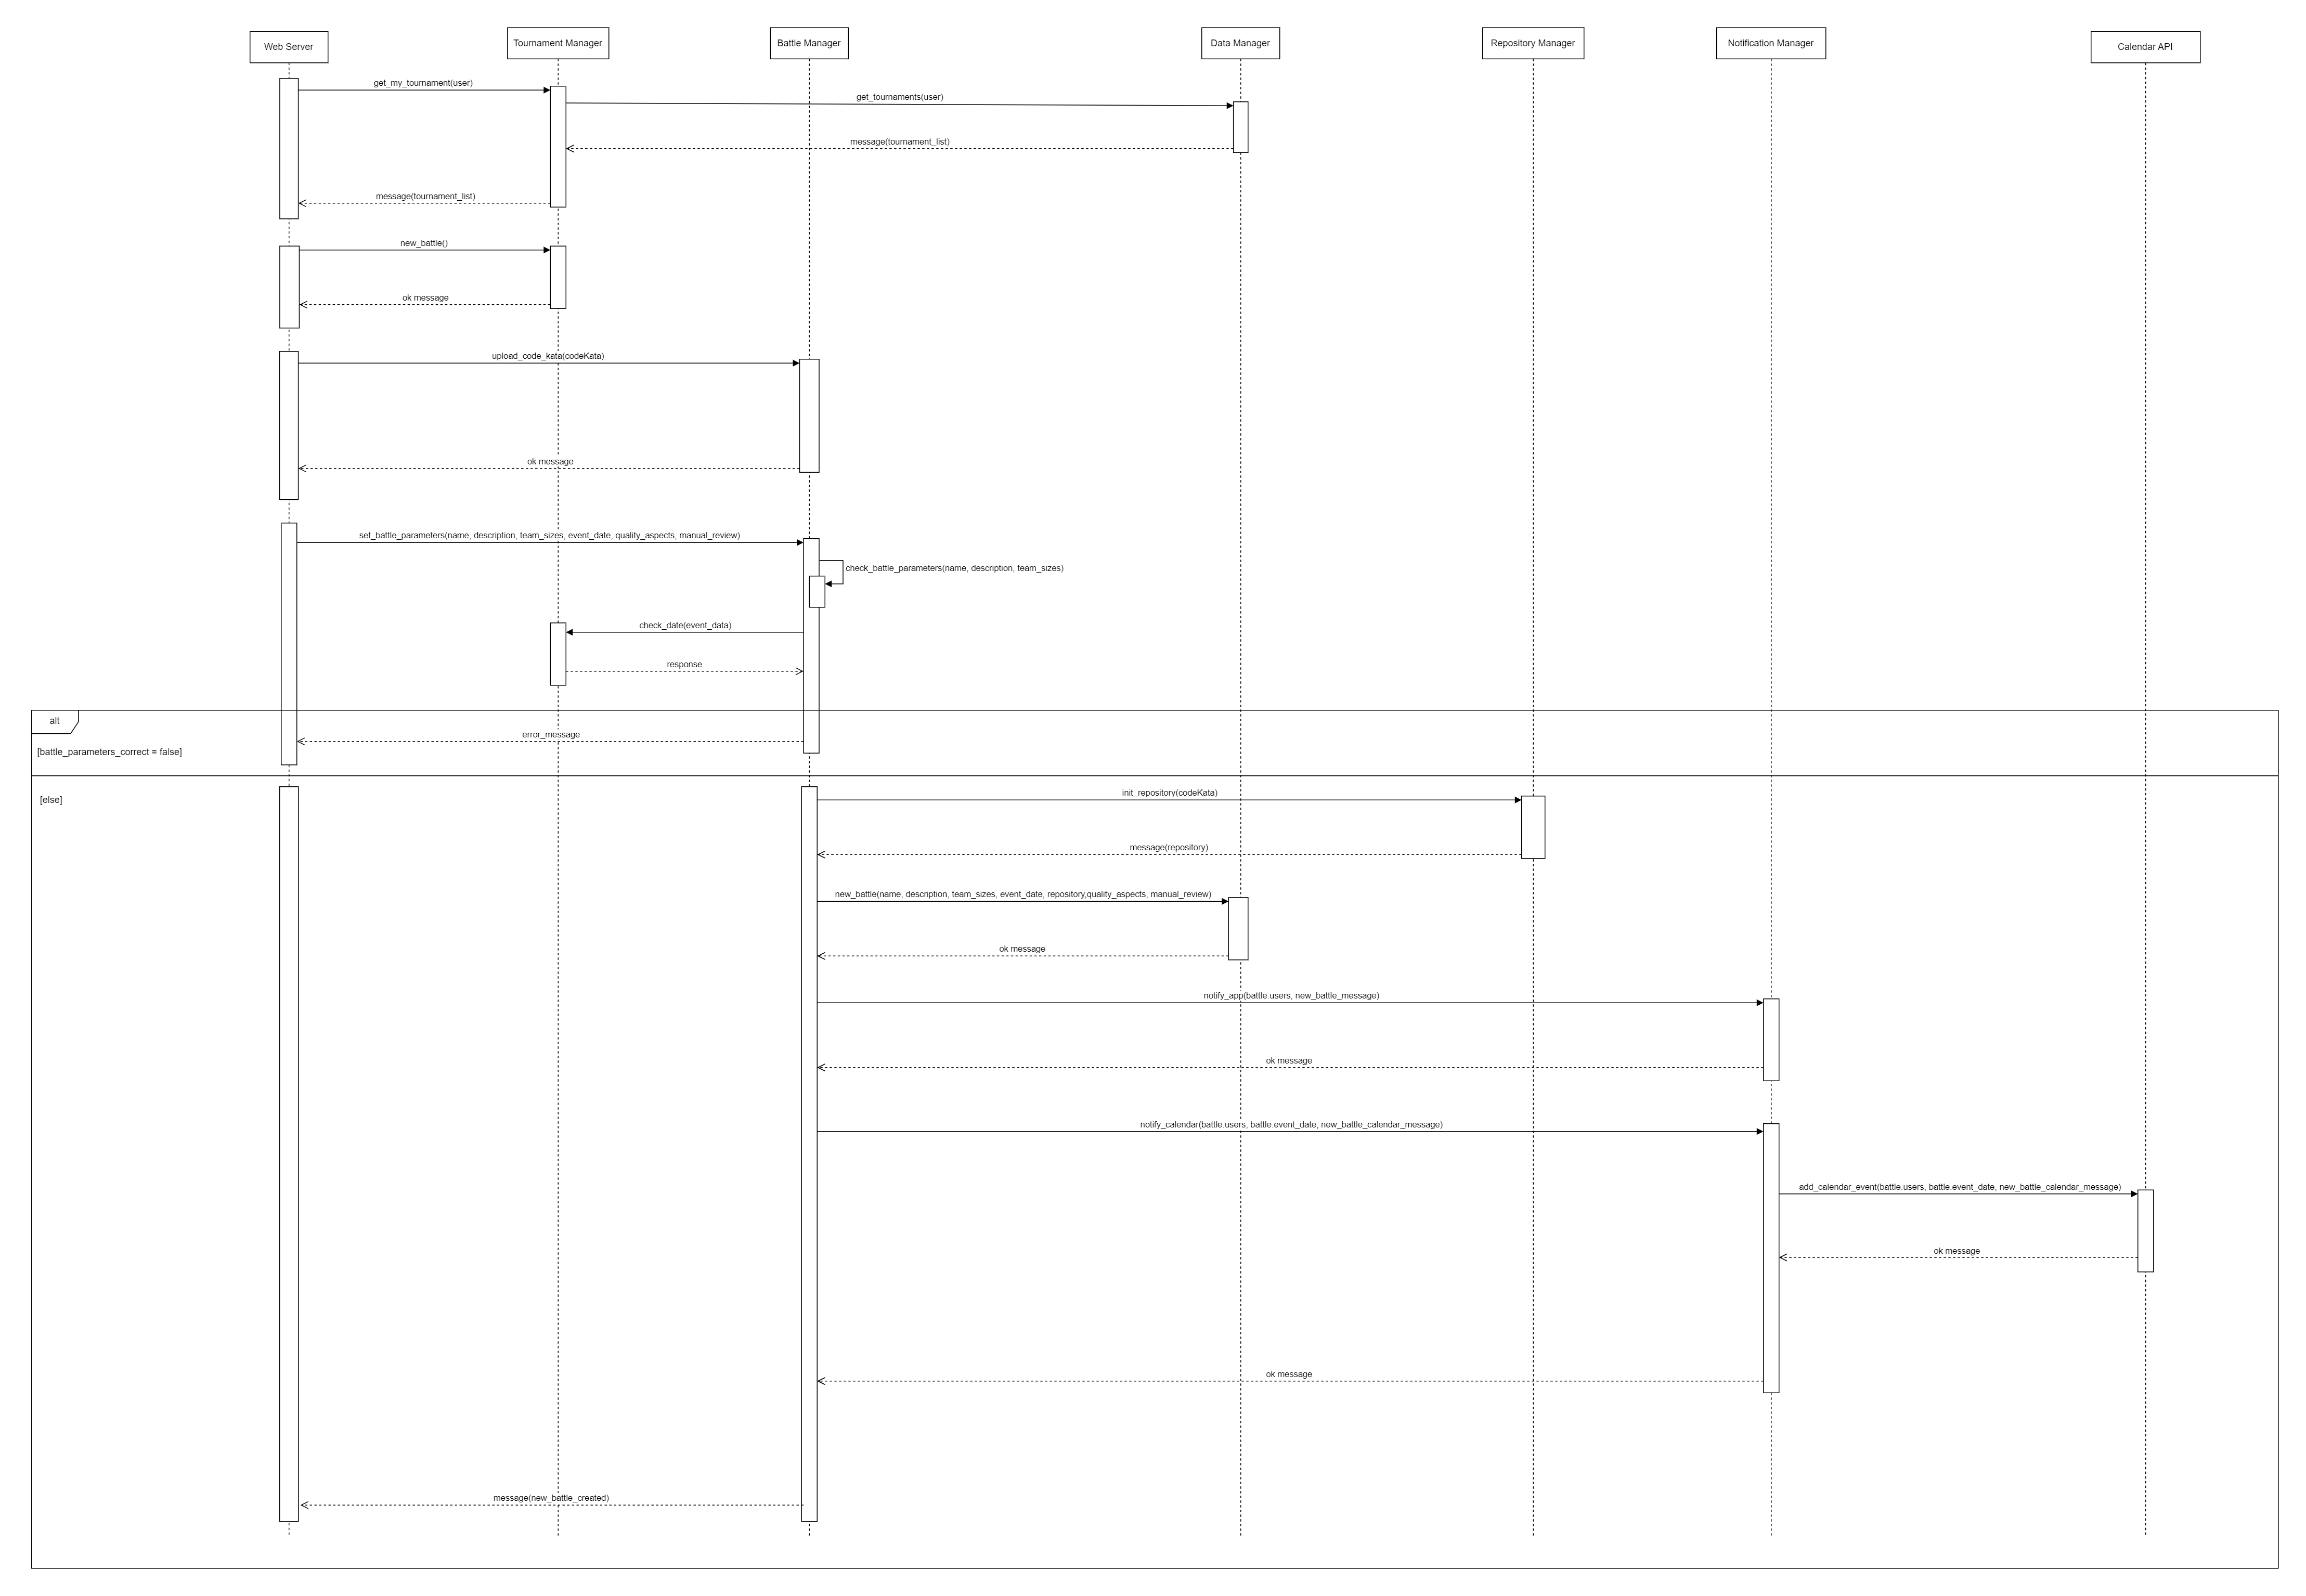
\includegraphics[width=1.4\textwidth]{../assets/section_2/CreateABattle.png}
    \end{figure}
    The \textit{Create a battle} phase involves an educator entering the battle's information into the designated fields.
    In this phase the educators sets all the constraints for the battle, including the CodeKata, the deadlines, the maximum number of participants, and the automated evaluations settings.
    Before creating the battle, the system checks that the all the provided information is valid and consistent(e.g. the deadline is after the start date).
    Upon successful verification a new battle is created and a notification is sent to all the students subscribed to the tournament where the battle belongs.
    \newpage

    \textbf{Subscribe to a tournament}\\
    \begin{figure}[H]
        \centering
        \hspace*{-3cm}
        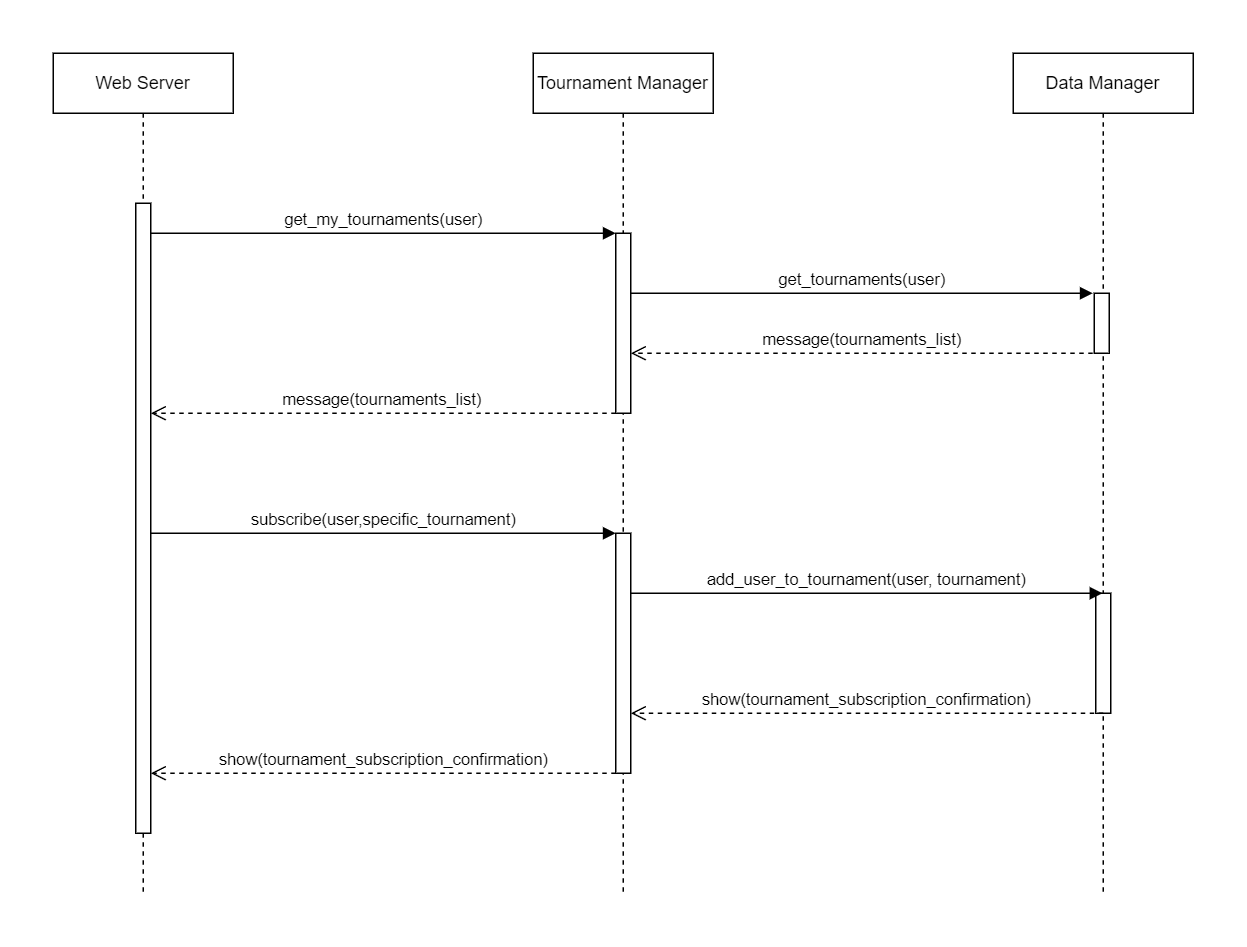
\includegraphics[width=1.35\textwidth]{../assets/section_2/SubscribeToATournament.png}
    \end{figure}
    The \textit{Subscribe to a tournament} phase involves a student selecting a tournament from the list of available tournaments in which he/she wants to participate.
    Upon a successful subscription, the user, now student, is eligible to enroll in the battles of the tournament. 
    \newpage

    \textbf{Create a group}\\
    \begin{figure}[H]
        \centering
        \hspace*{-3cm}
        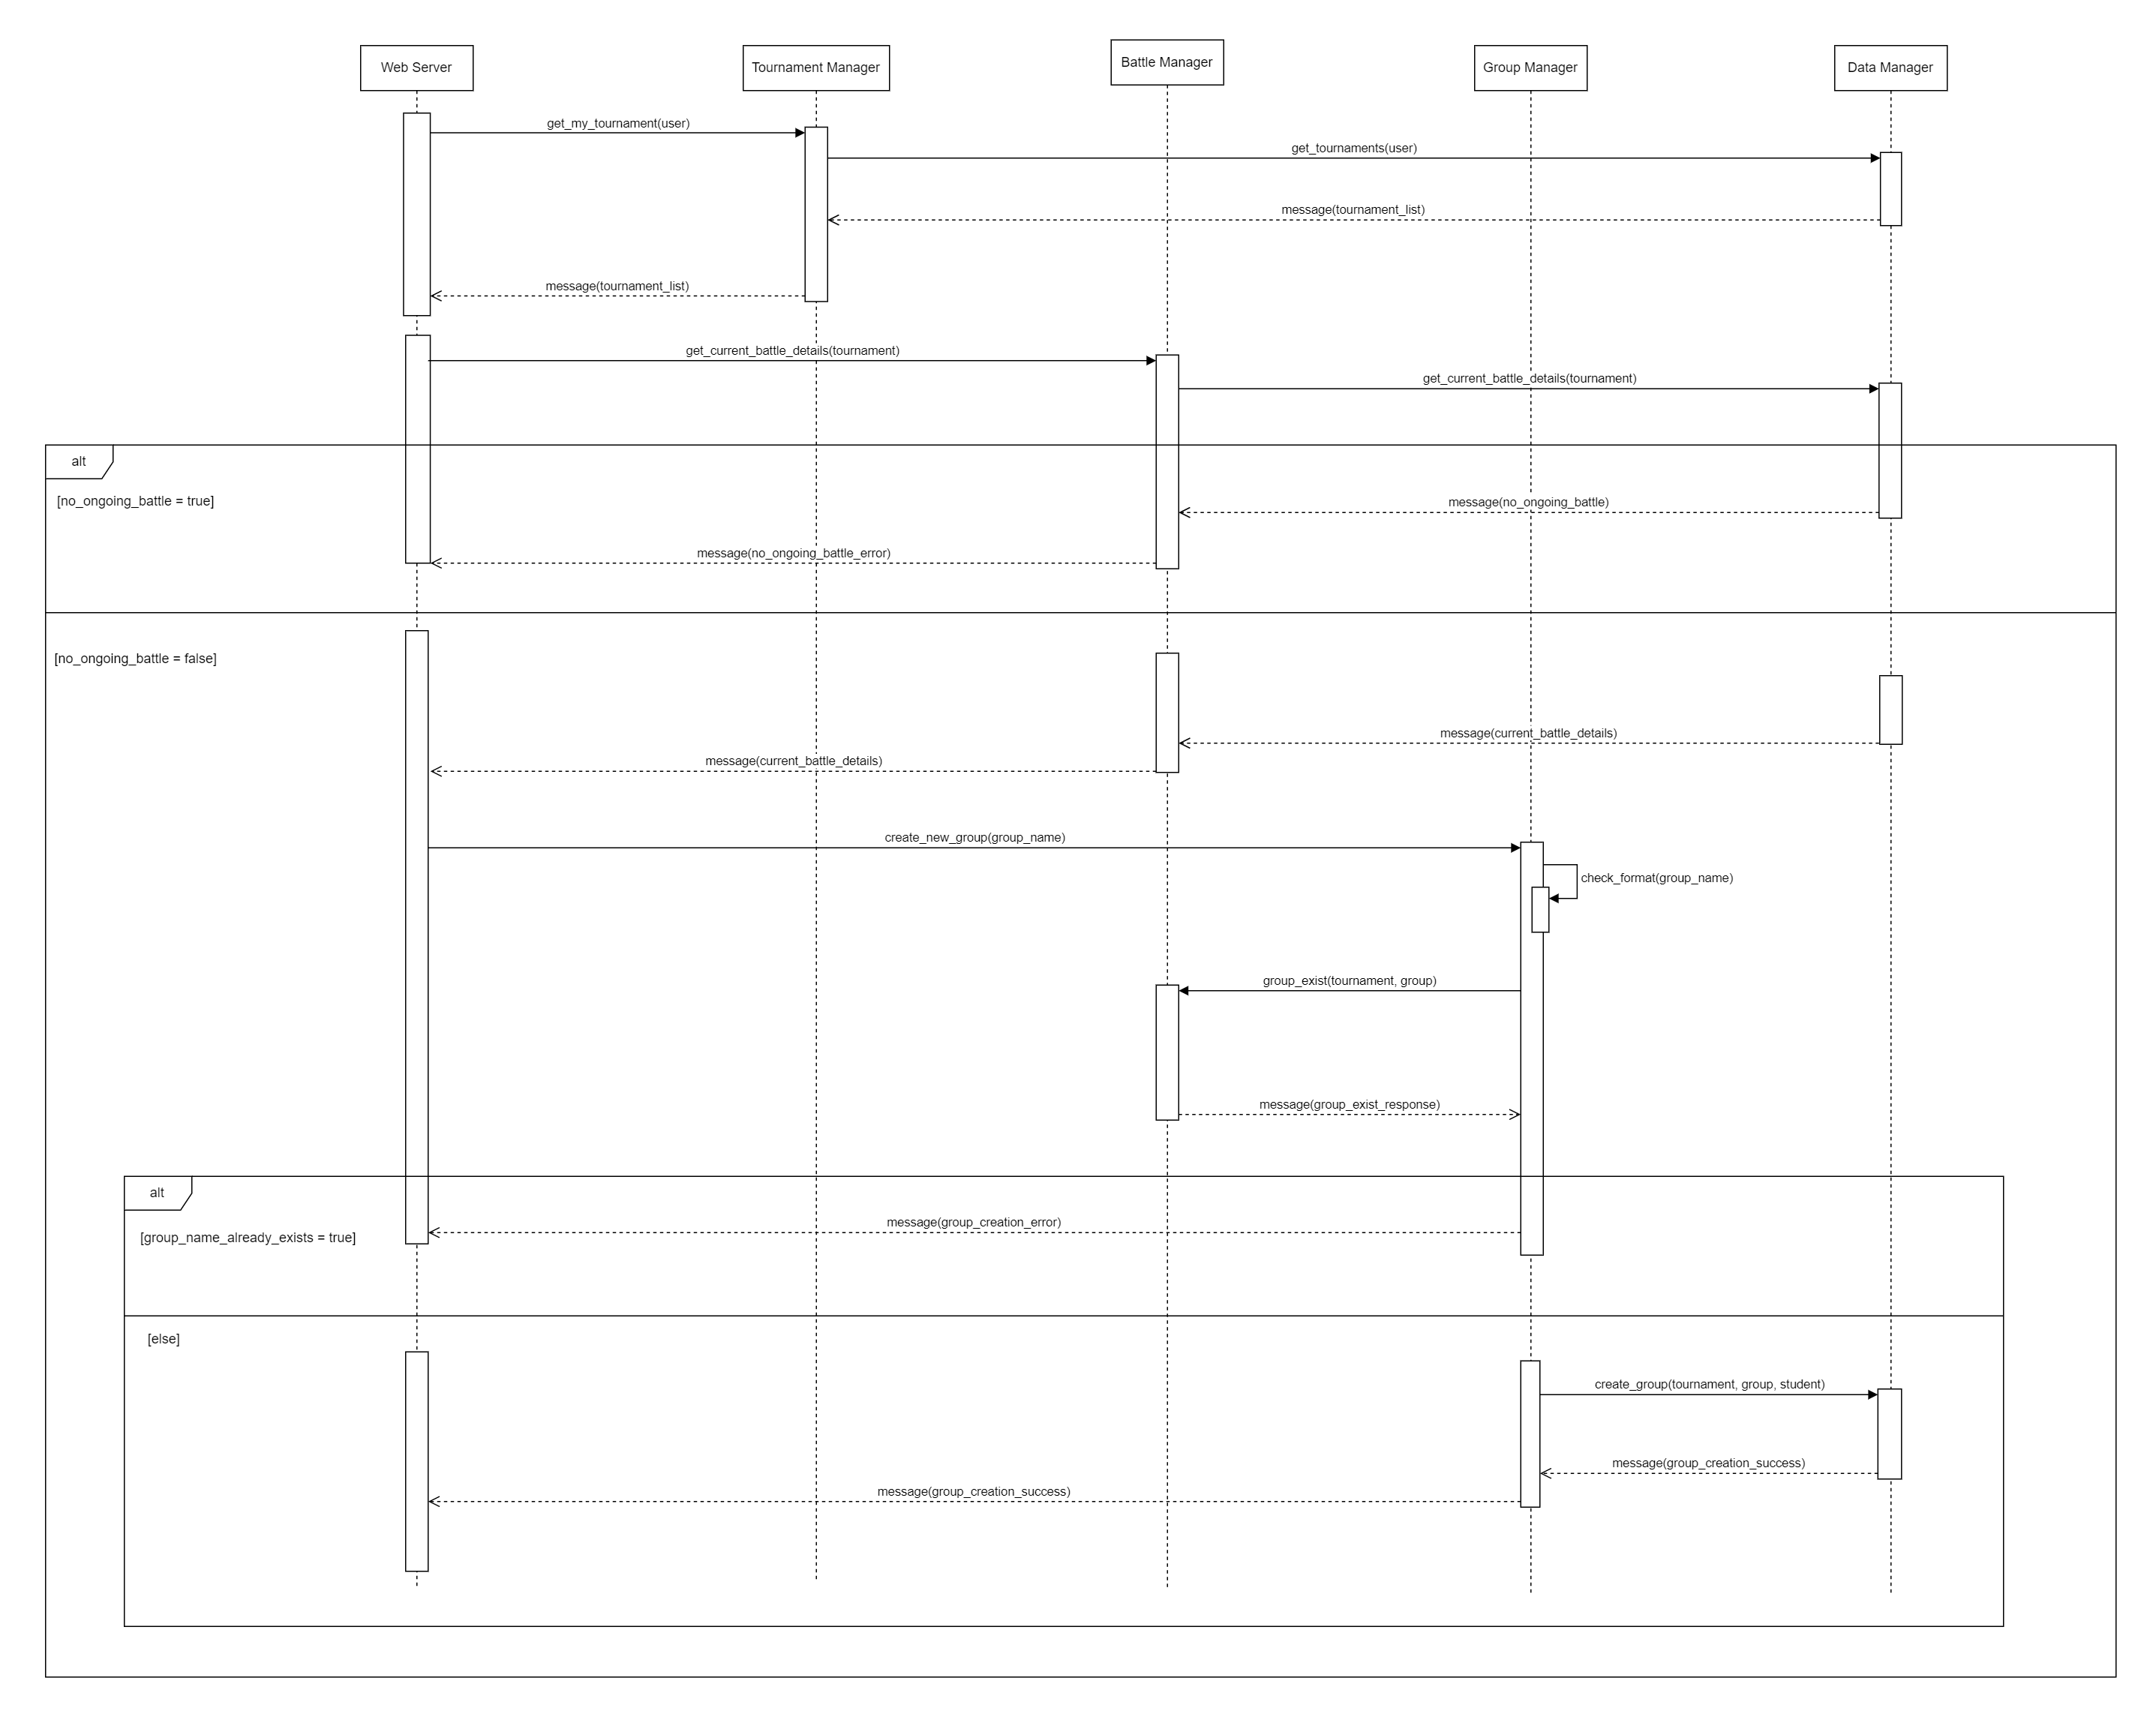
\includegraphics[width=1.4\textwidth]{../assets/section_2/CreateAGroup.png}
    \end{figure}
    The \textit{Create a group} phase involves a student creating a new group in order to compete with other colleagues to battles.
    To do so the student has to provide the name of the group using the provided field.
    The system checks that no other group has the same name in the context of the battle in which the student is going to create such a group.
    \newpage

    \textbf{Invite a student to an existing group}\\
    \begin{figure}[H]
        \centering
        \hspace*{-3cm}
        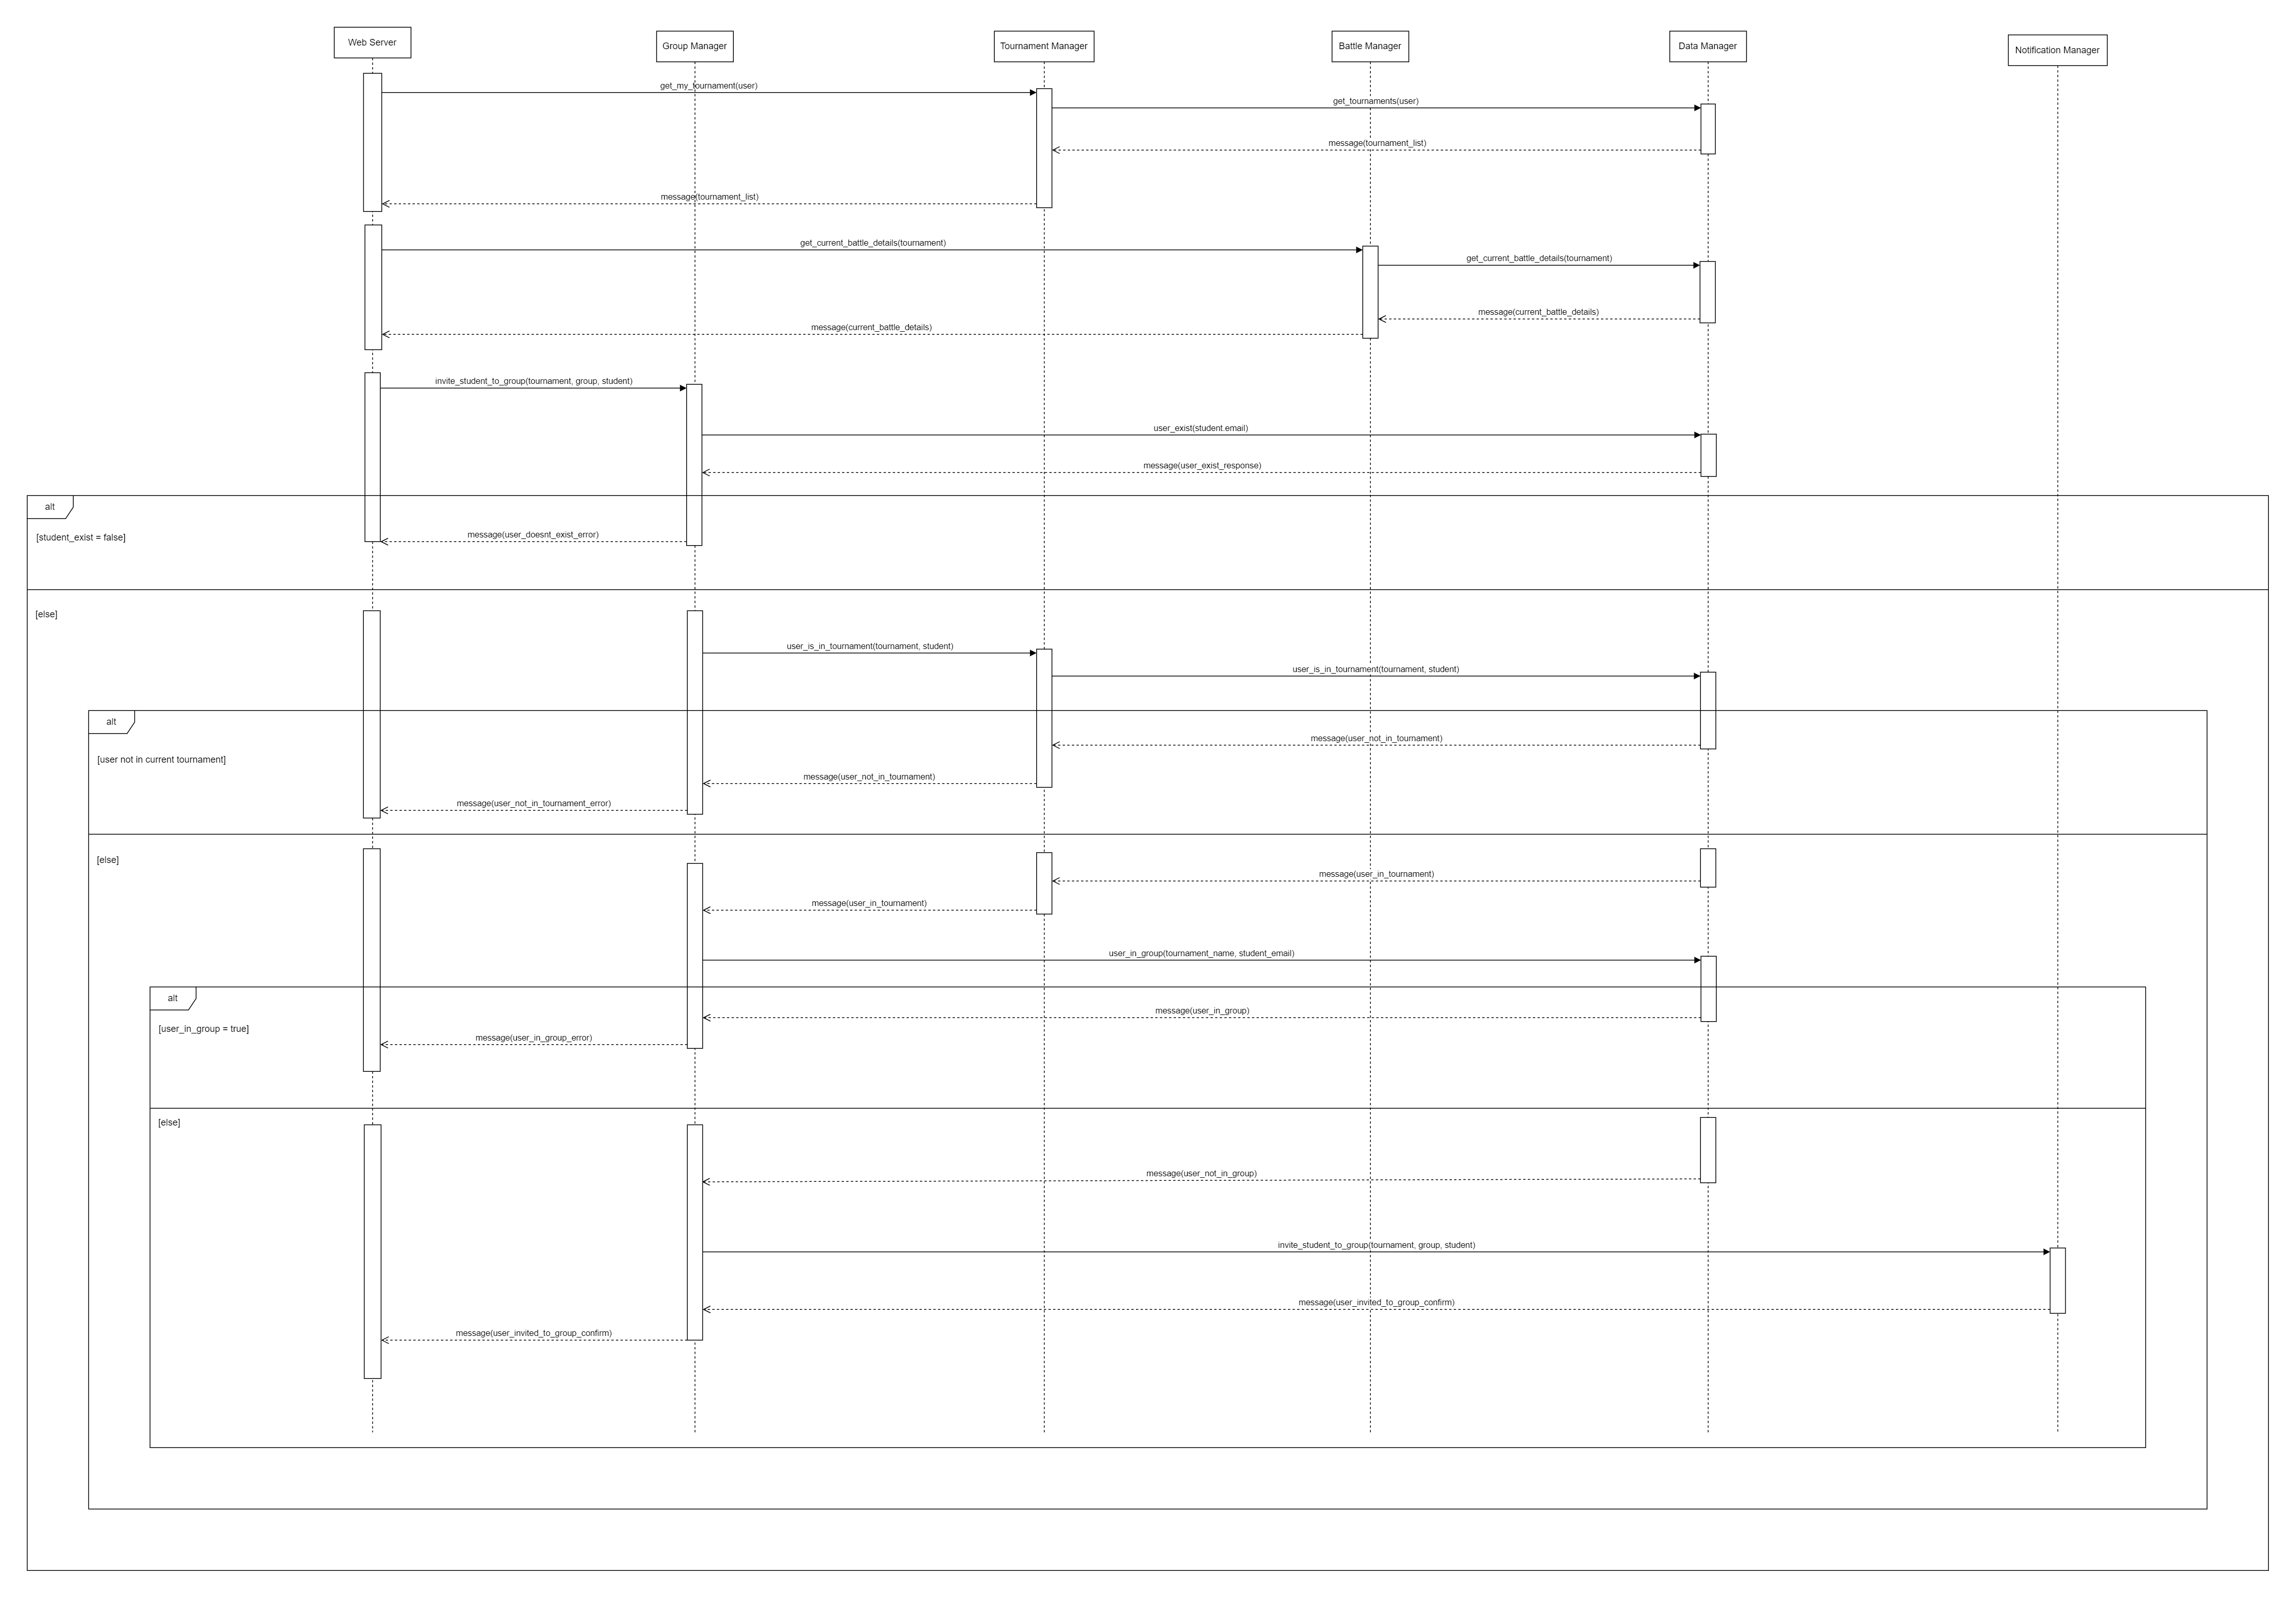
\includegraphics[width=1.4\textwidth]{../assets/section_2/InviteStudentsToExistingGroup.png}
    \end{figure}
    \newpage
    The \textit{Invite a student to an existing group} phase involves a student inviting another student to join an existing group.
    In particular, the system checks:
    \begin{itemize}
        \item {if the invited student exists;}
        \item {if the invited student is enrolled in the same tournament and battle as the inviting student;}
        \item {if the invited student is already enrolled in another group in the same battle.}
    \end{itemize}
    Upon successful verification of the aforementioned conditions a notification is sent to the invited student.
    \newpage

    \newgeometry{top = 3em}
    \textbf{Enroll in a battle}
    \begin{figure}[H]
        \centering
        \hspace*{-2cm}
        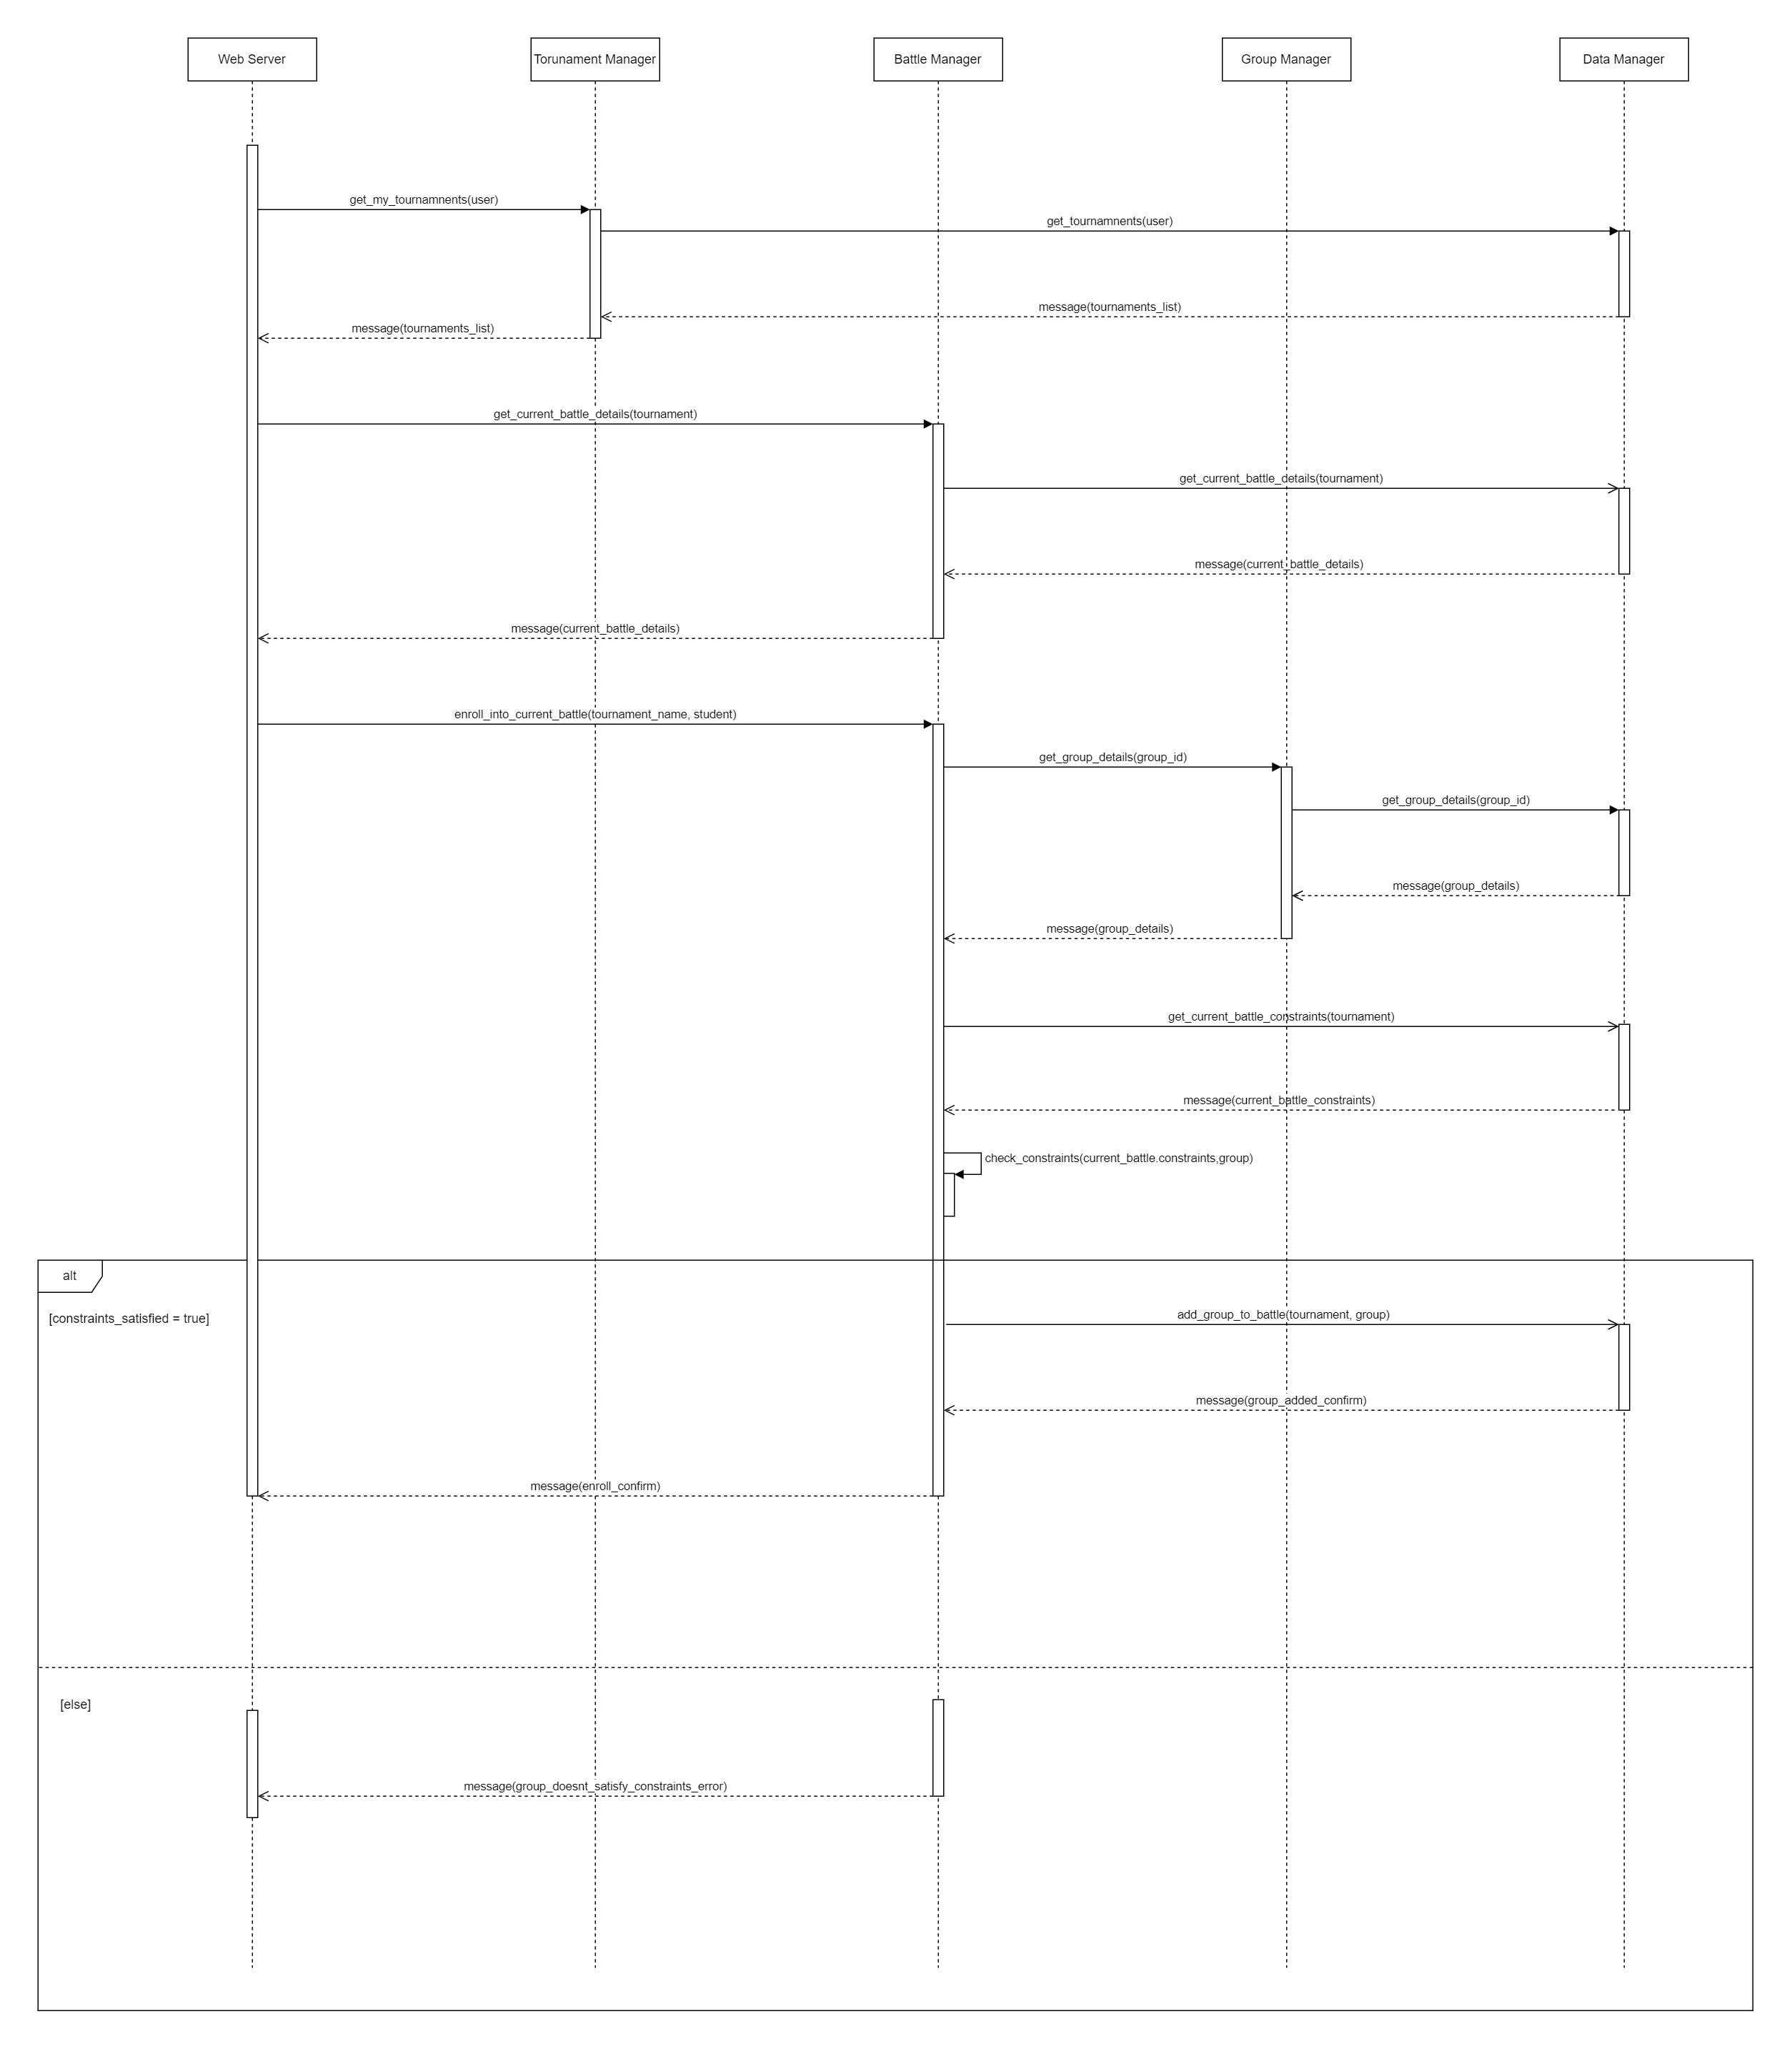
\includegraphics[width=1.15\textwidth]{../assets/section_2/EnrollInABattle.png}
    \end{figure}
    The \textit{Enroll in a battle} phase involves a student enrolling in a battle.
    In this stage the system ensures that the group enrolling in the battle has the correct size. Upon successful check the student is enrolled in the battle and can compete.
    \restoregeometry
    \newpage

    \textbf{Student delivers a solution}\\
    \begin{figure}[H]
        \centering
        \hspace*{-3cm}
        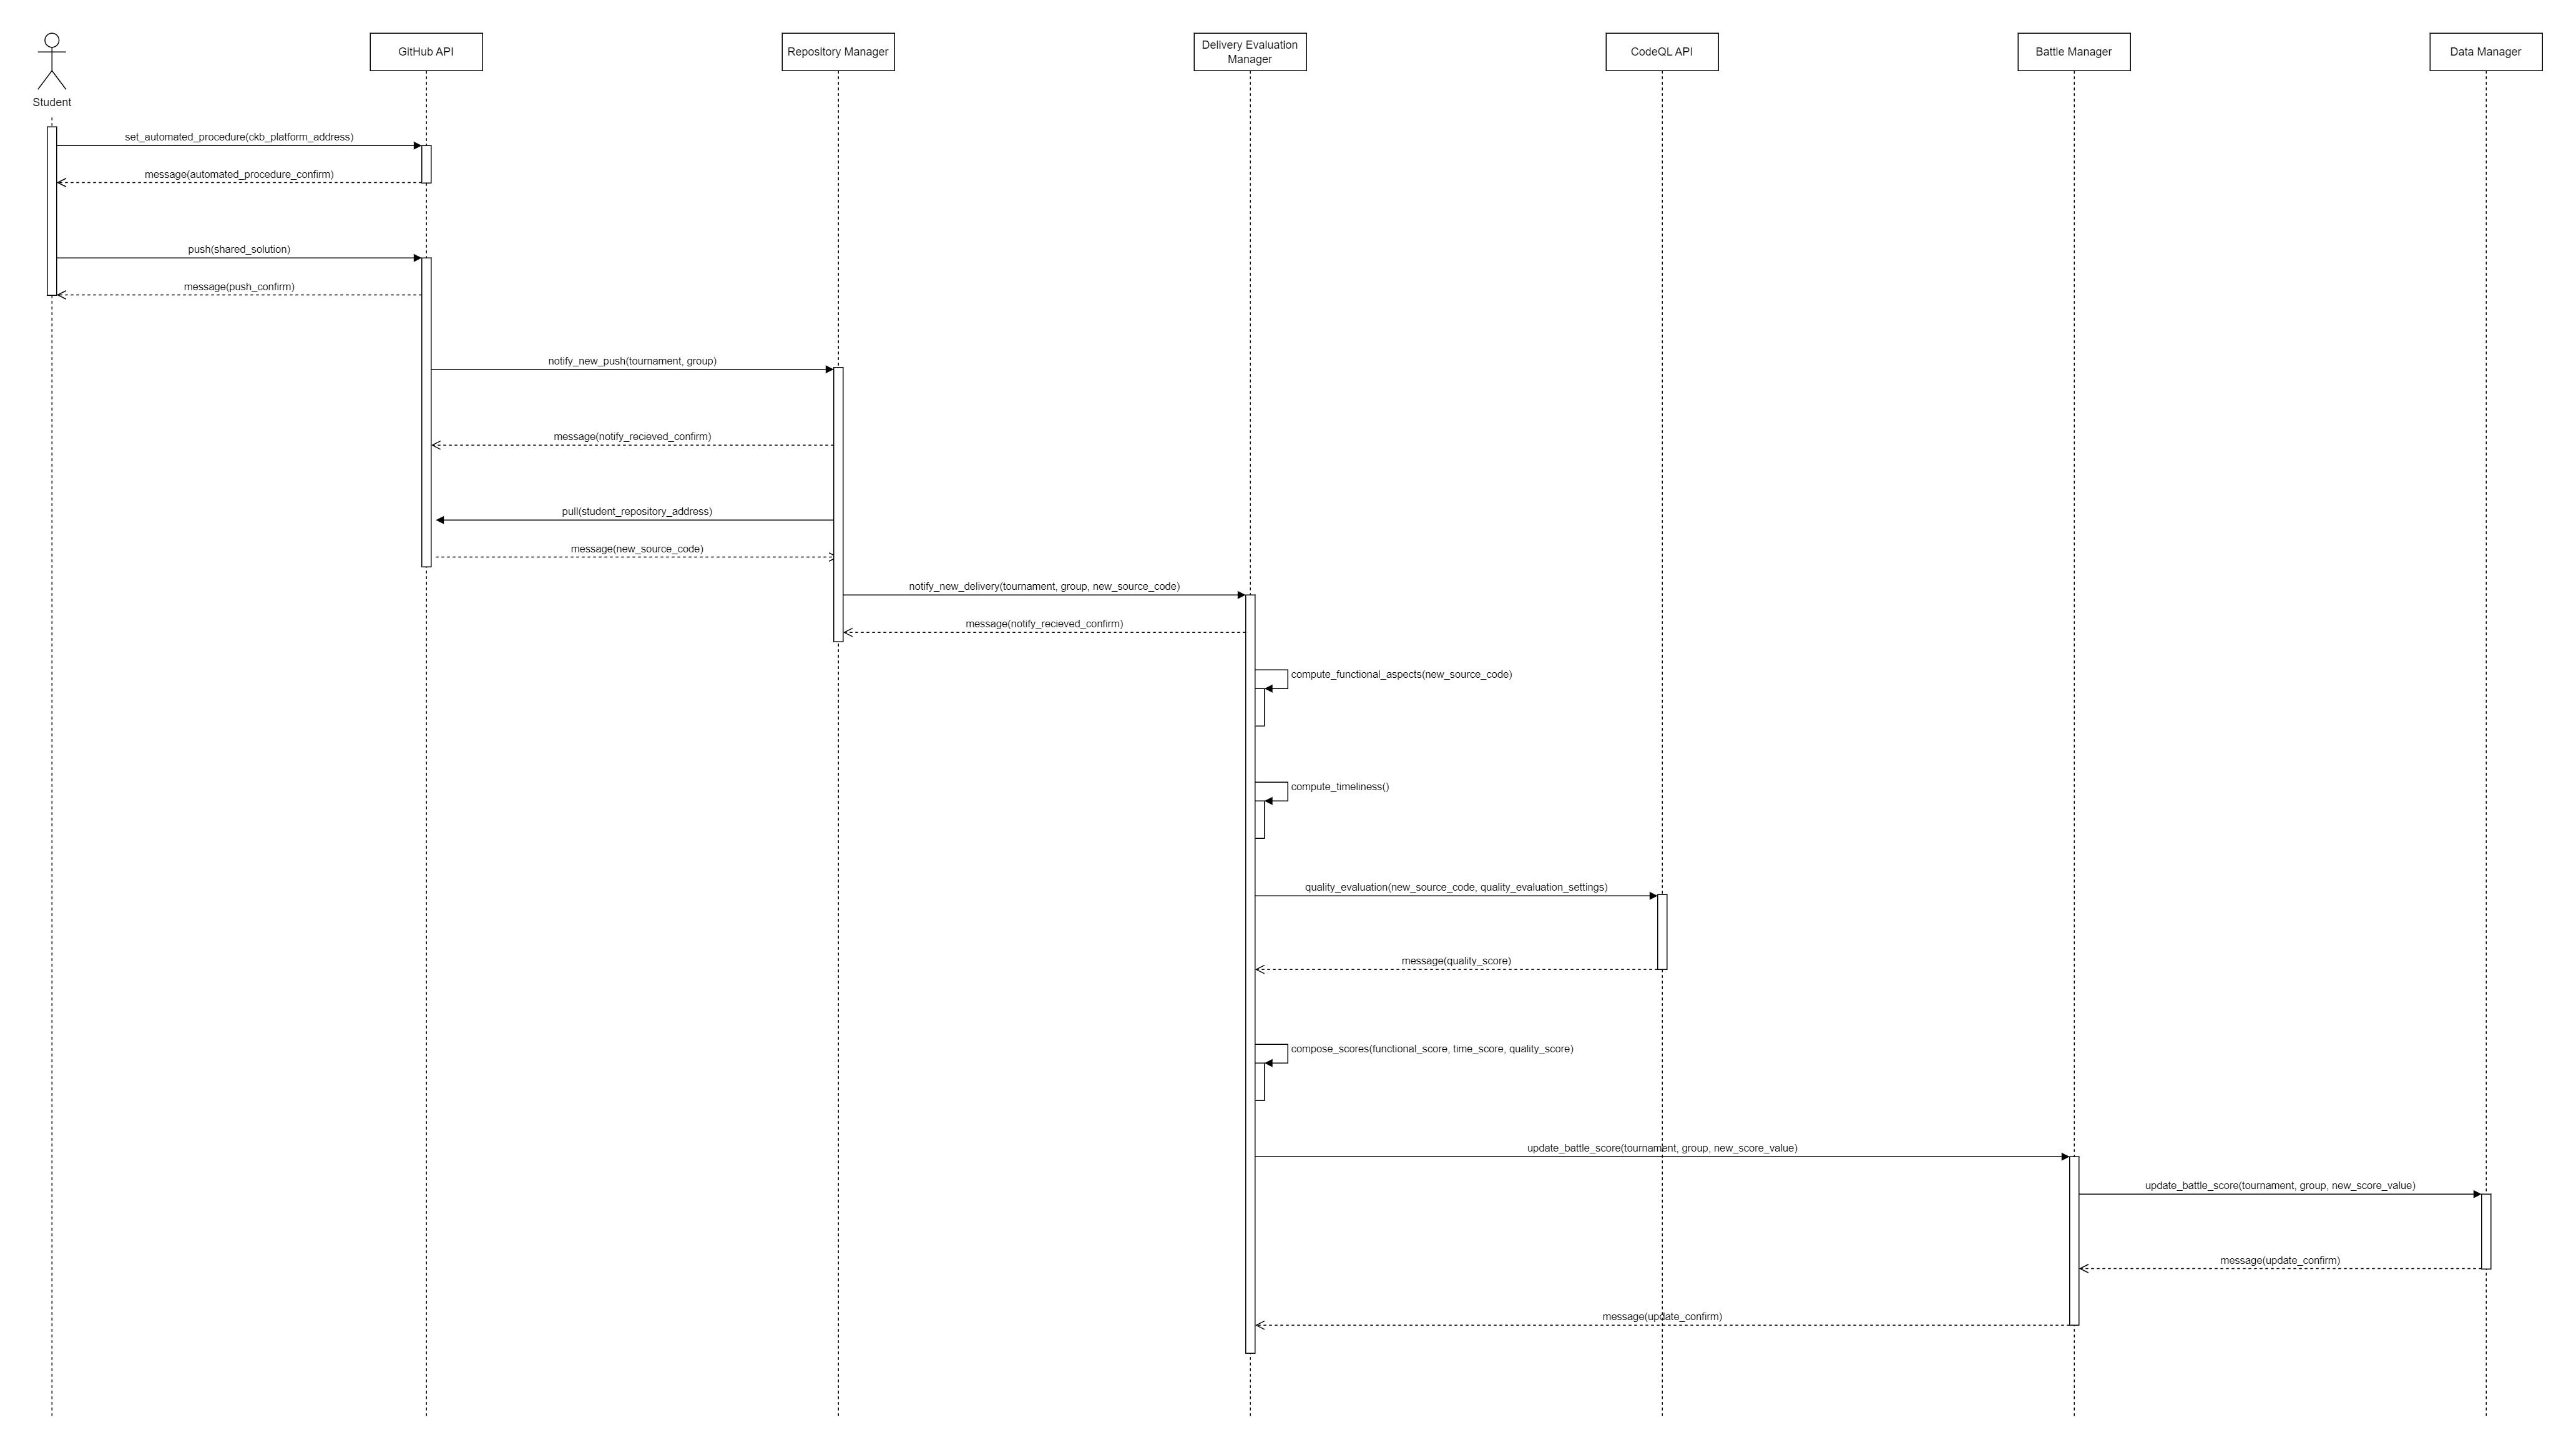
\includegraphics[width=1.4\textwidth]{../assets/section_2/StudentDeliversASolution.png}
    \end{figure}
    The \textit{Student delivers a solution} phase involves a student delivering a solution to a battle.
    In this phase, after the student has pushed the solution to the online repository, the system automatically evaluates the solution according to the criteria set by the educator in the battle configuration.
    The solution is first evaluated in terms of timeliness and number of passed test.
    A second code quality evaluation is performed by \textit{CodeQL}\footnote{CodeQL is a semantic code analysis engine that allows to write queries to find vulnerabilities in code} based on the battle settings.
    In order for this procedure to be successful the user has to set up an automated workflow using \textit{GitHub Actions}.
    \newpage

    \textbf{Educator does a manual code review}
    \begin{figure}[H]
        \centering
        \hspace*{-3cm}
        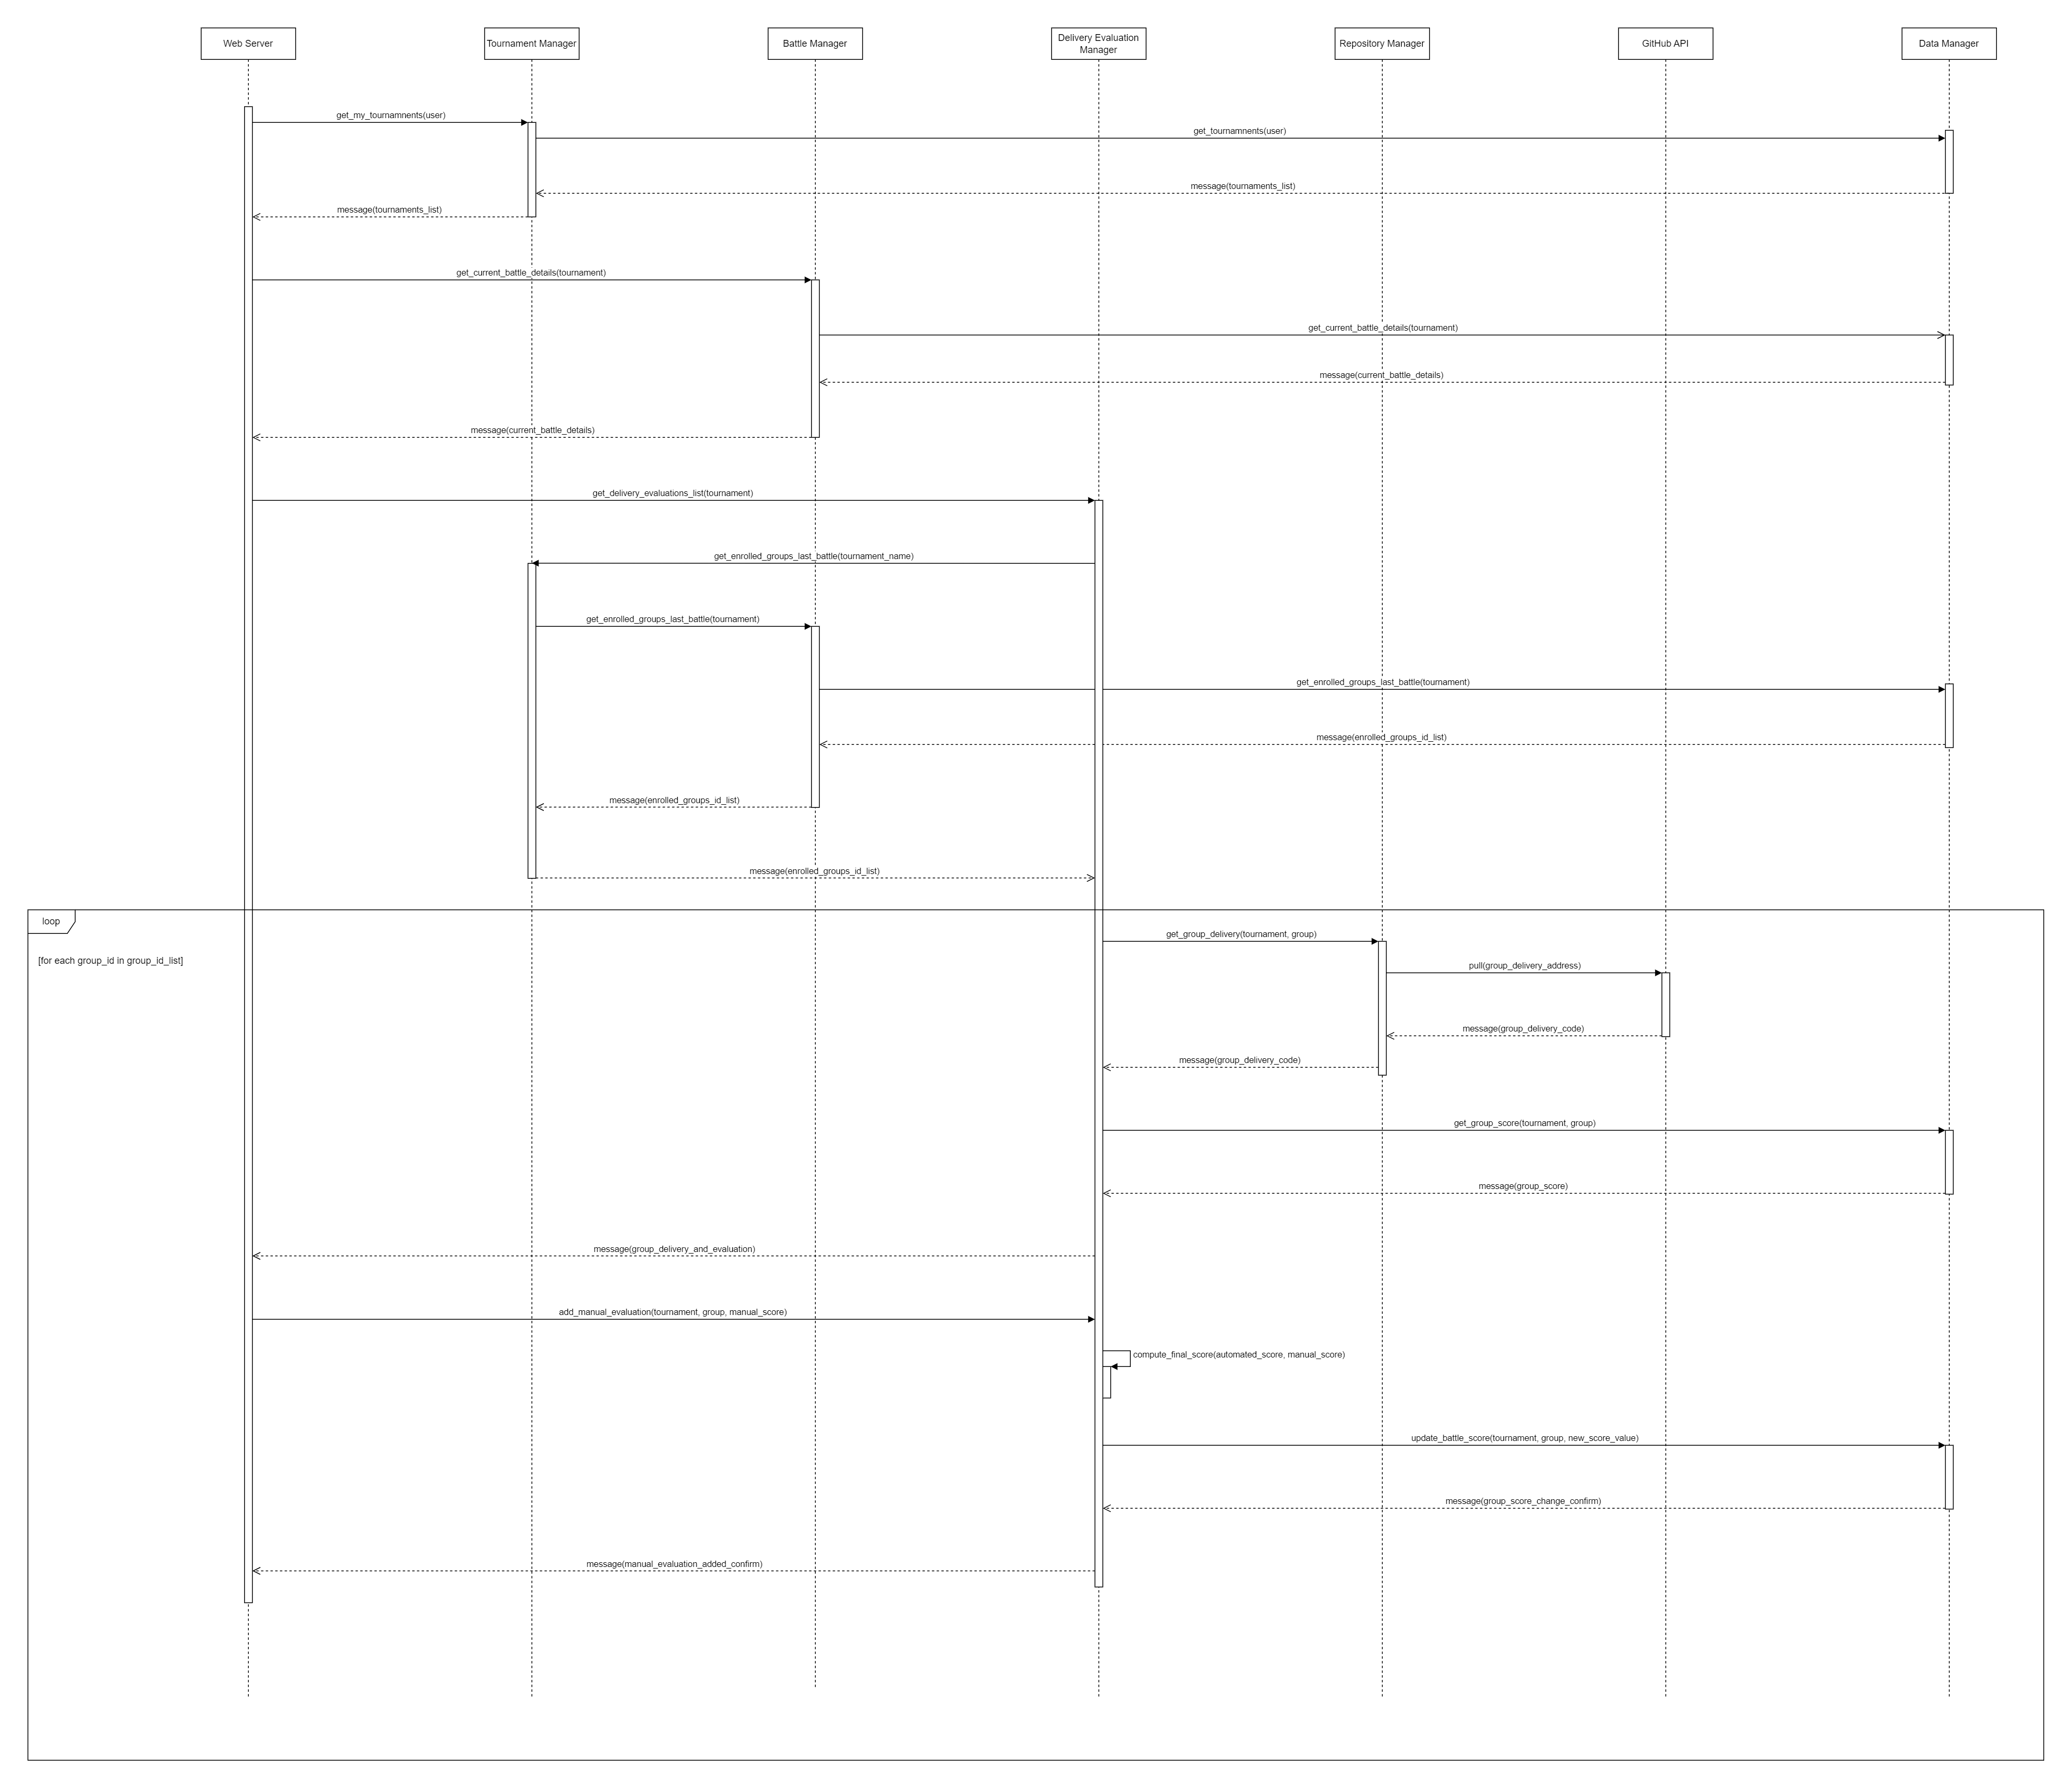
\includegraphics[width=1.4\textwidth]{../assets/section_2/EducatorDoesAManualCodeReview.png}
    \end{figure}
    \newpage
    The \textit{Educator does a manual code review} phase involves an educator reviewing a student's solution.
    In this procedure, after the \textit{Student delivers a solution} phase, the educator can manually evaluate the solution.
    The solution score is updated starting from the automated evaluation score.
    It's important to note that the manual review does not substitute the automated one, but it's rather a complement to it that aims to fix, at some extent, the initial automated one.
    \newpage

    \textbf{Close a battle early}\\
    \begin{figure}[H]
        \centering
        \hspace*{-3cm}
        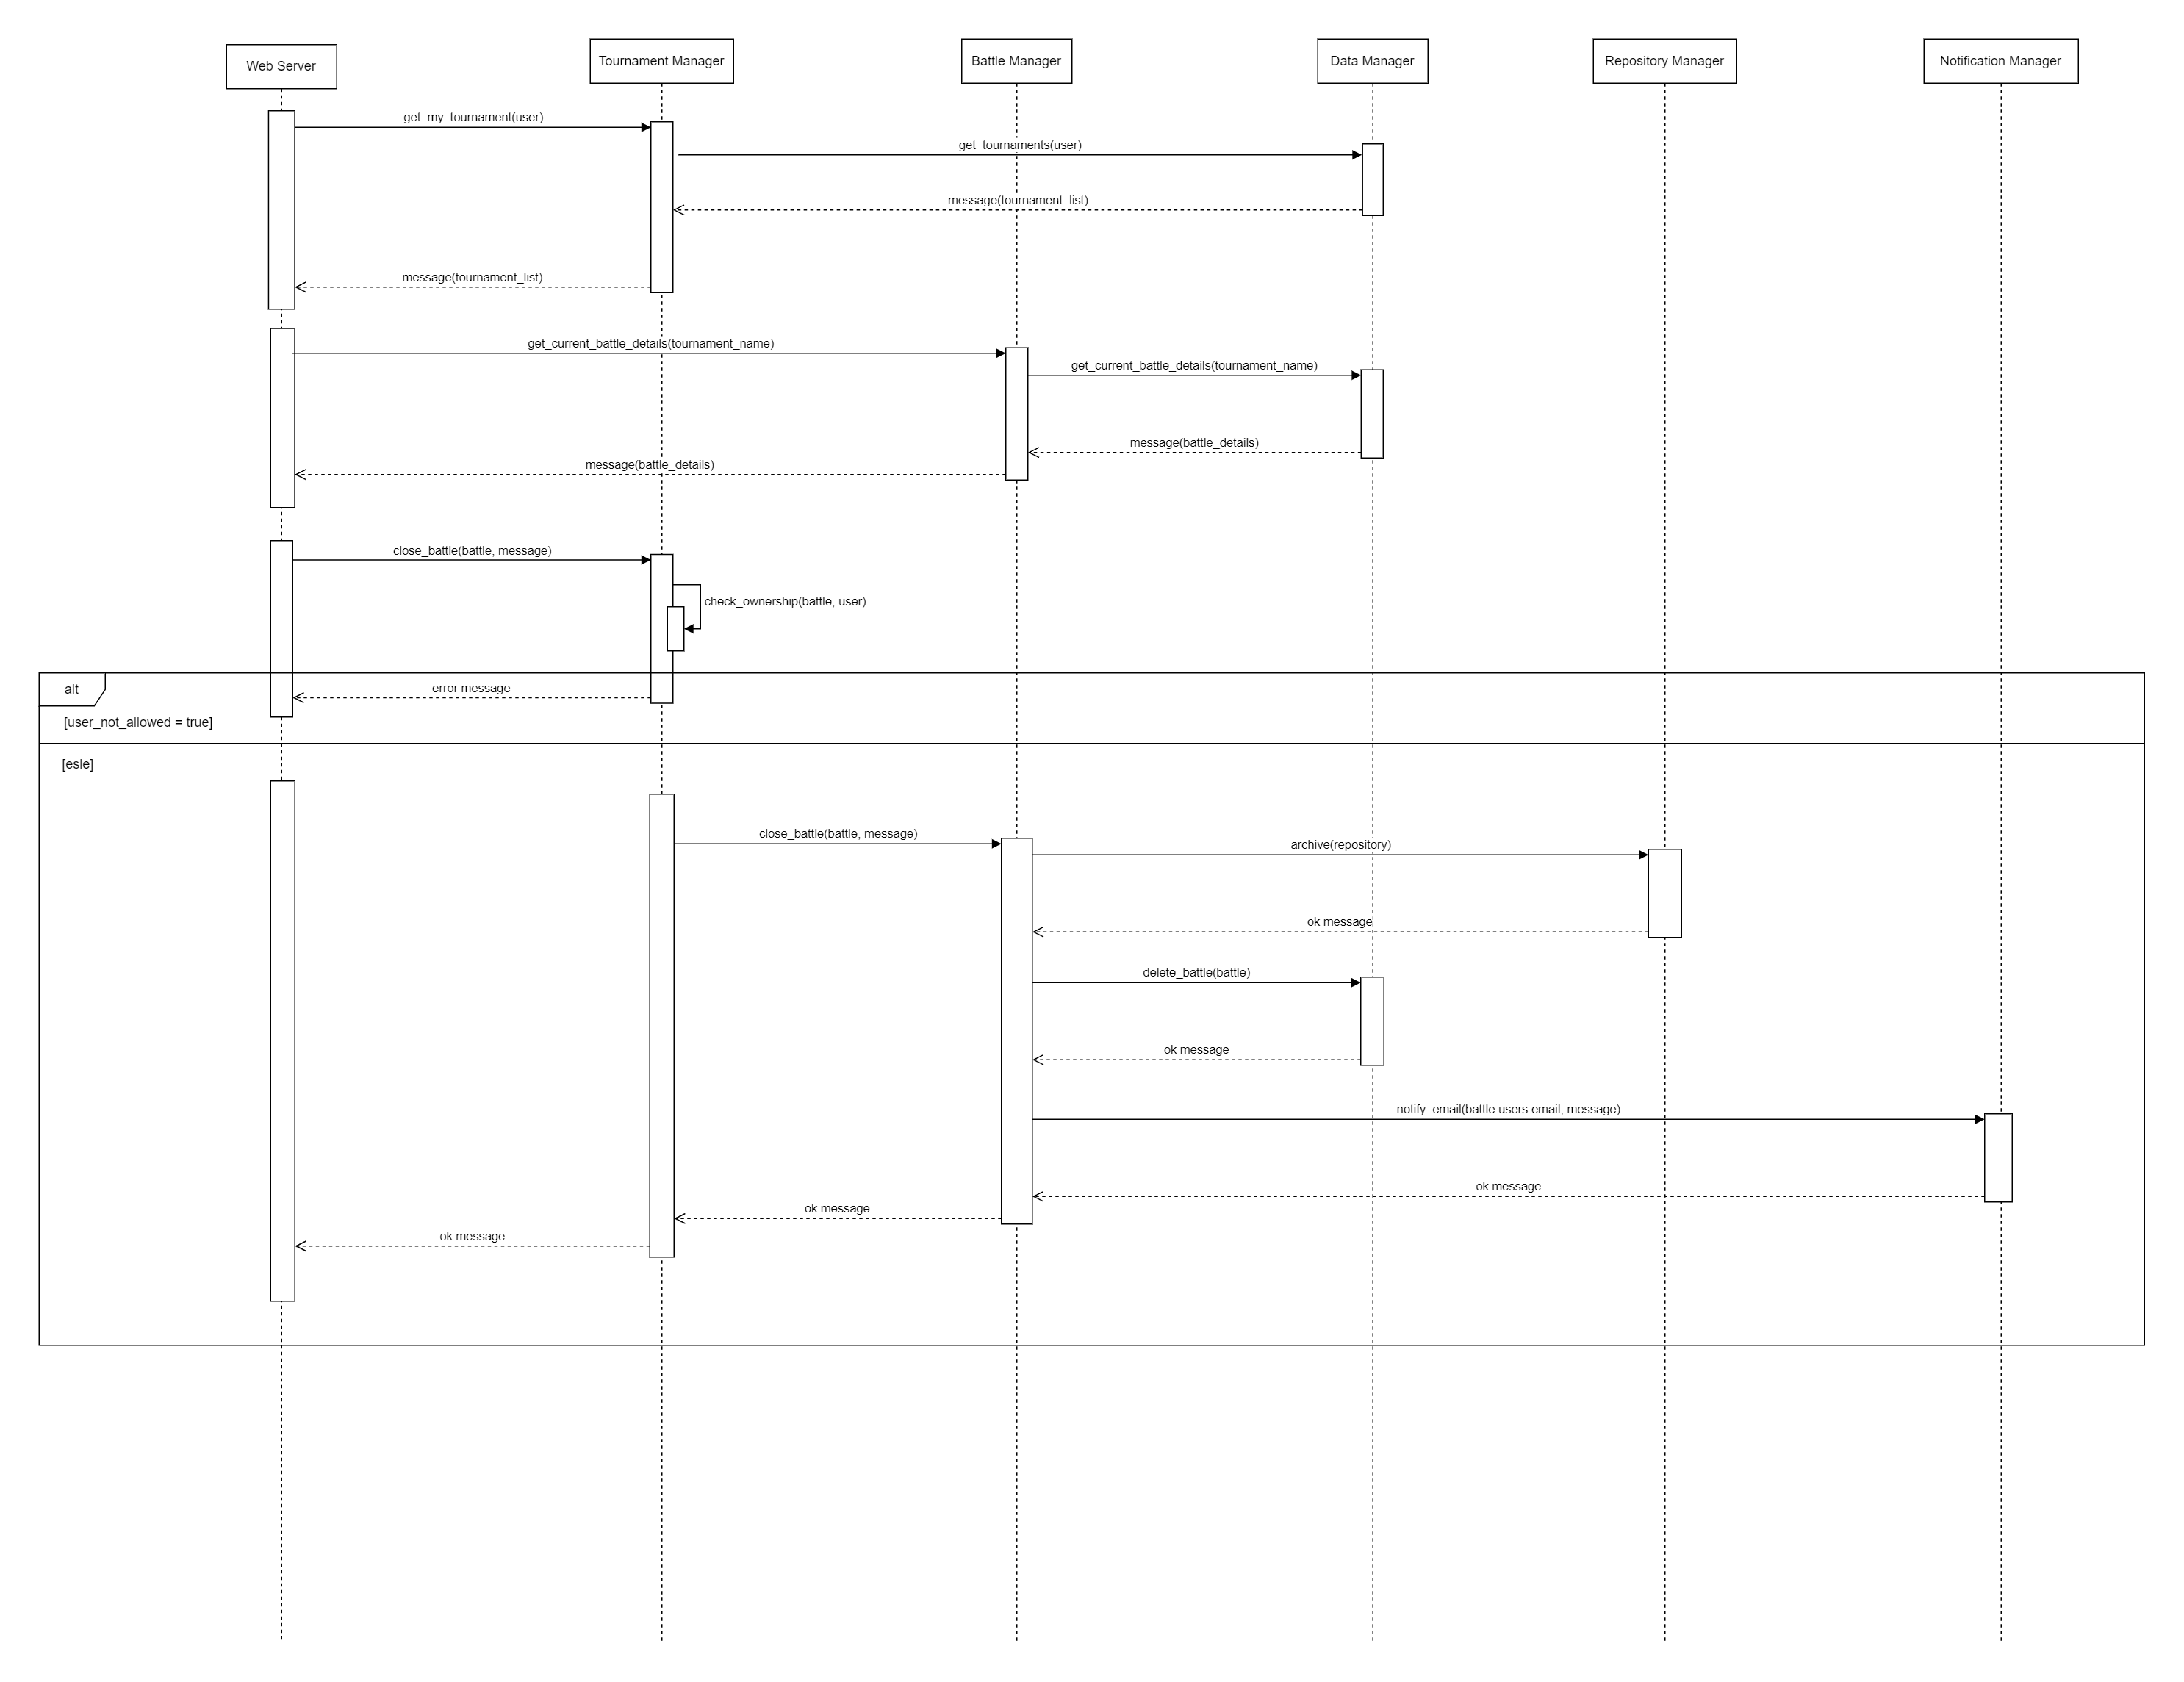
\includegraphics[width=1.4\textwidth]{../assets/section_2/CloseABattle.png}
    \end{figure}
    \newpage
    The \textit{Close a battle early} phase involves an educator closing a battle before the deadline.
    In this phase the system checks that the educator has the ownership, hence the permission to close the battle.
    Upon successful verification the system closes the battle by deleting it from the database and archiving the corresponding CodeKata repository.
    The educator, using the provided field, also needs to specify a reason for the early closure of the battle, which will be included in the notification sent to all the previously subscribed students.
    \newpage

    \textbf{Close a tournament}\\
    \begin{figure}[H]
        \centering
        \hspace*{-3cm}
        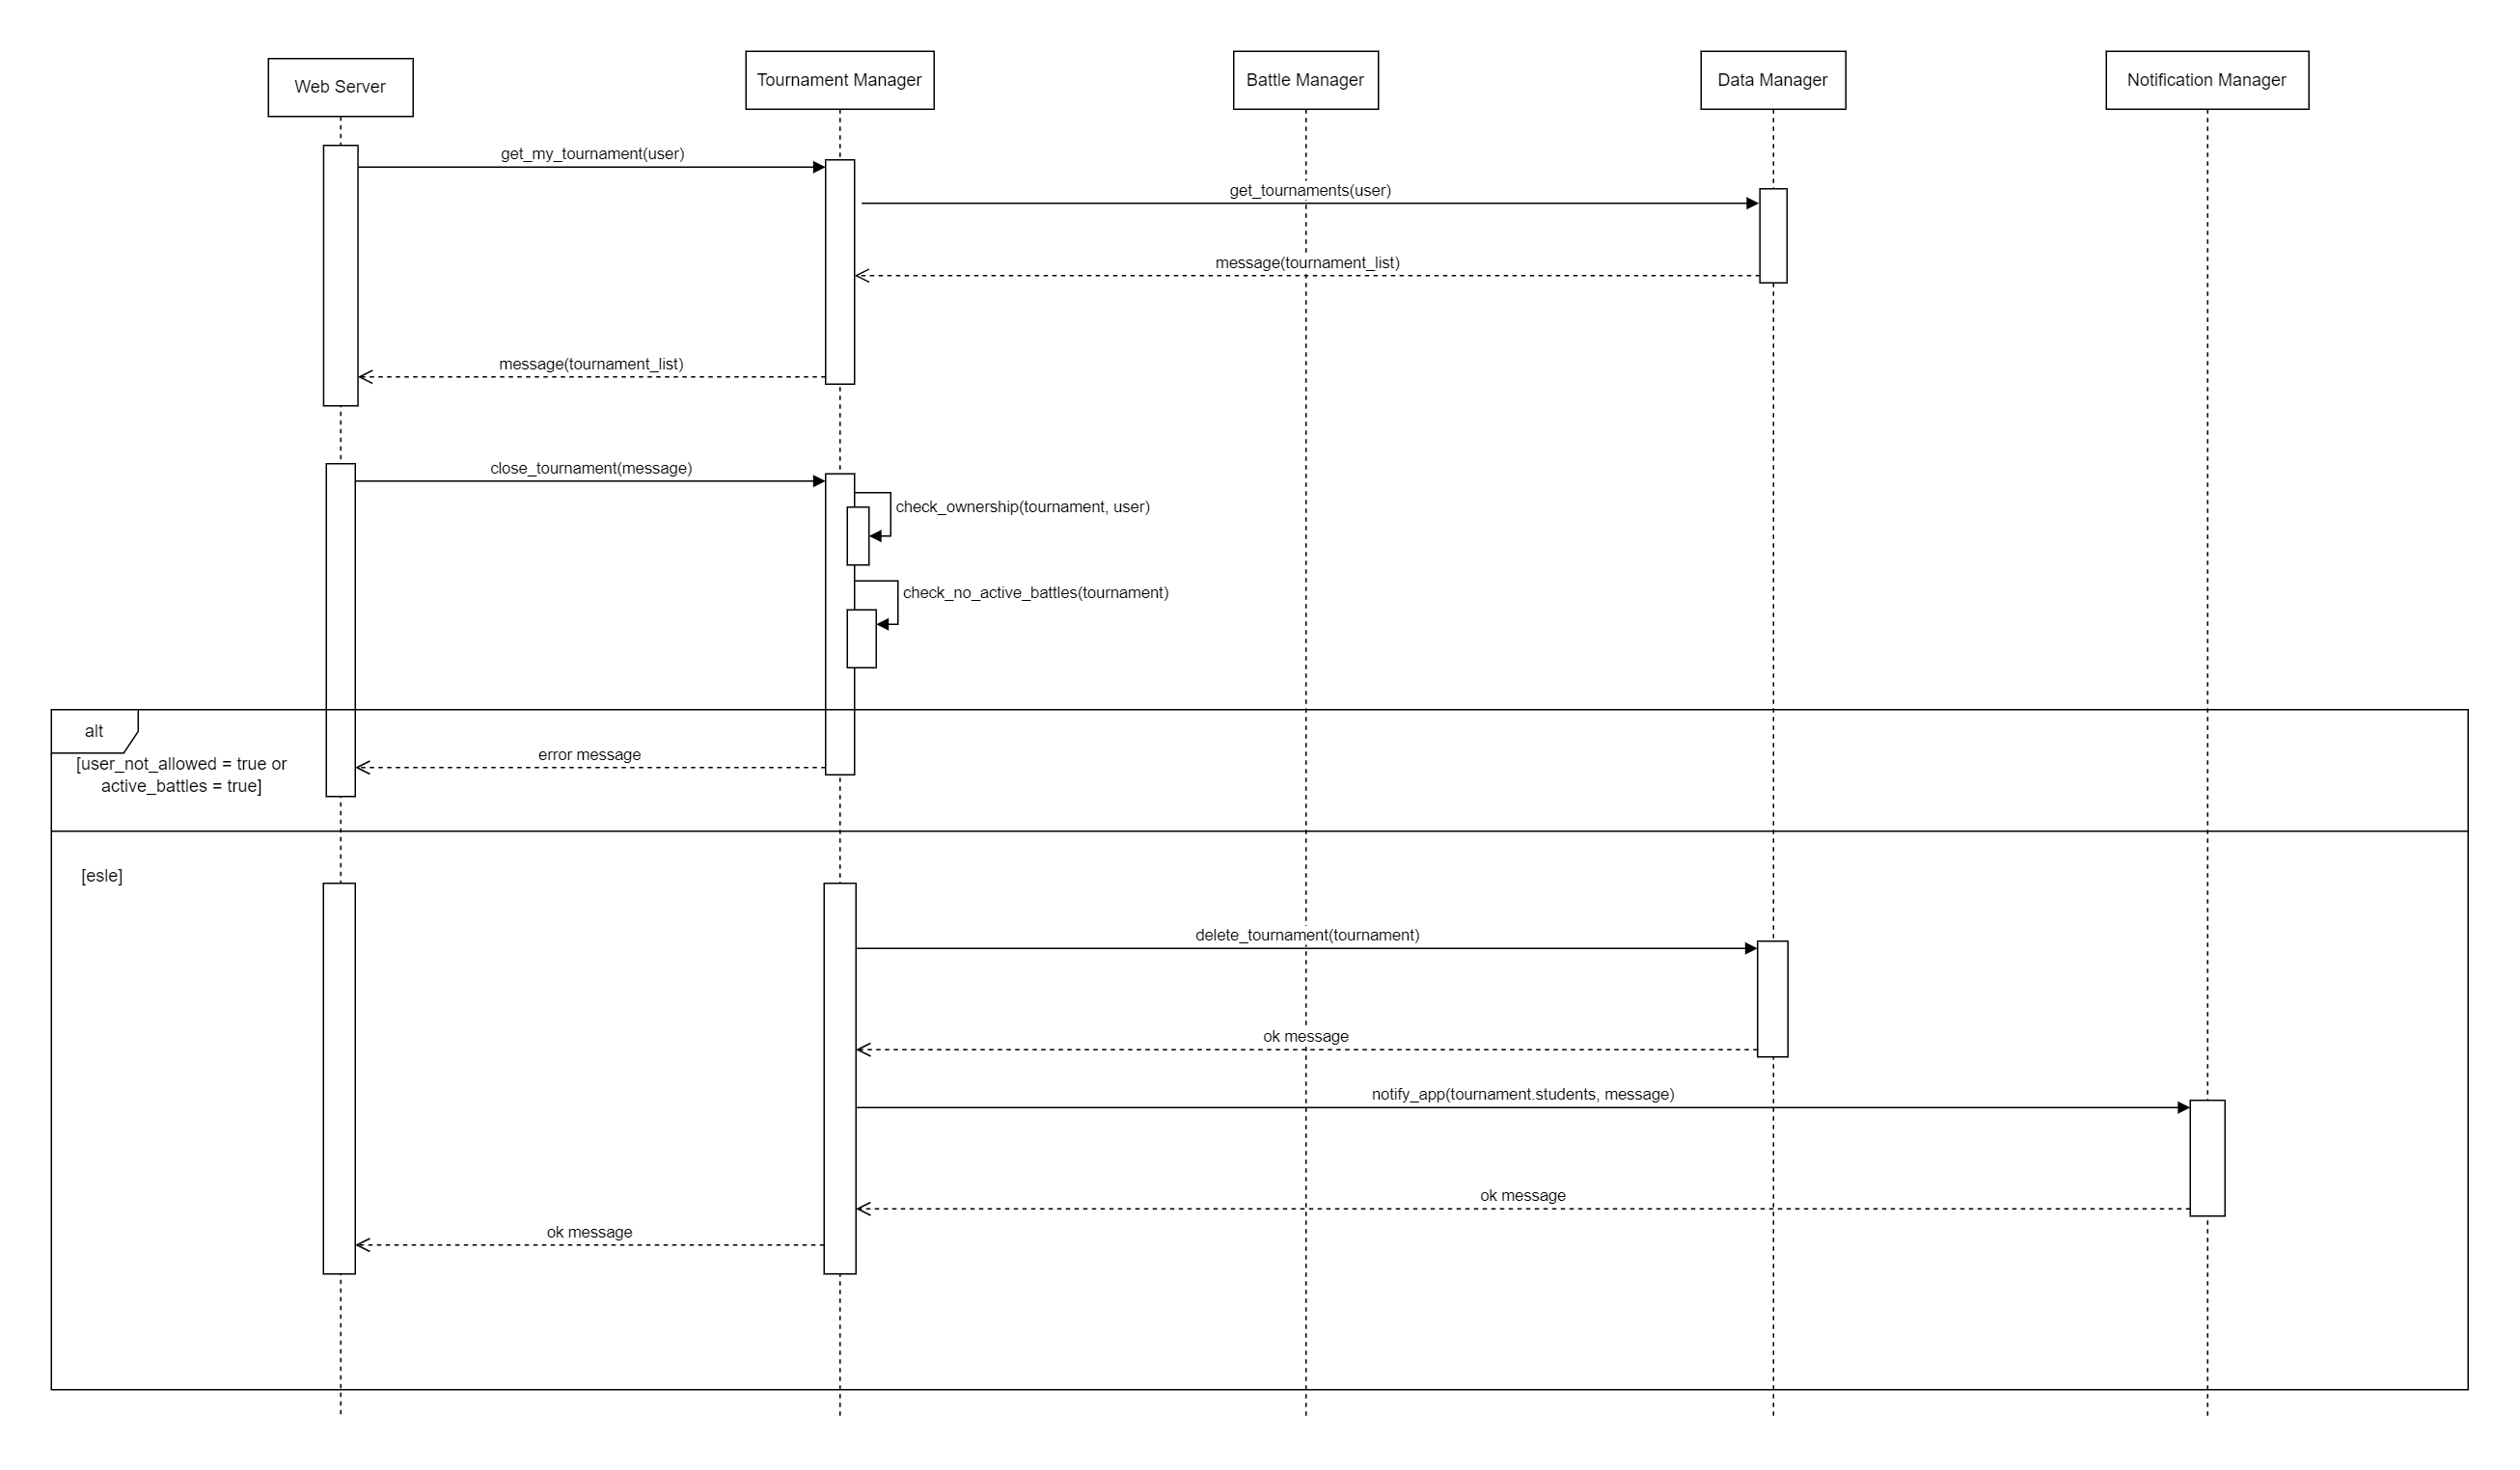
\includegraphics[width=1.4\textwidth]{../assets/section_2/CloseTournament.png}
    \end{figure}
    The \textit{Close a tournament} phase involves an educator closing a tournament.
    In this state, the systems checks that no battles are still ongoing in such a tournament.
    Upon successful check the system closes the tournament by deleting it from the database.
    A notification informing the students of the tournament's closure is sent to all the previously subscribed students.
    \newpage

    \subsection{Selected Architectural Styles and Patterns}\label{subsec:selected_architectural_styles_and_patterns}
    Here below are discussed the utilized architectural styles and patterns:
    \begin{itemize}
        \item {\textbf{Three Tier Architecture}: The chosen system architecture is a three-tier architecture comprising a presentation tier, a logic tier, and a data tier.
        \begin{itemize}
            \item {The \textit{presentation tier} is responsible for presenting the application to the user and for handling user interaction;}
            \item {The \textit{logic tier} processes the input, performing necessary calculations or operations necessary to the correct functioning of the application;}
            \item {The \textit{data tier} handles the storage and retrieval of data from a database.}
        \end{itemize}}
        \item {\textbf{Thin client}: The thin client approach enhances security by avoiding local storage of sensitive data and improves scalability by facilitating the deployment of new clients. 
        Additionally, it enables a more centralized management helpful in case of a dynamic environment where the application gets frequently updates.}
        \item {\textbf{Scalability}: The three-tier architecture enables a modular design, making it easier to scale individual components of the system. 
        Changes to one component do not necessarily require modifications to the other components.}
        \item {\textbf{Model-View-Controller}: The MVC design pattern is a software design pattern that divides an application into three primary components: the model, the view, and the controller. 
        The model constitutes the data and business logic, the view represents the user interface, and the controller facilitates communication between the model and the view. Specifically:
        \begin{itemize}
            \item {\textit{Model}: it's the central component of the pattern, serving as the dynamic data structure of the application. 
            The model is independent of the user interface, not concerned with how data is displayed nor how the user interacts with the application. 
            It directly manages the data, logic and rules of the application.}
            \item {\textit{View}: responsible for representing the user interface of the application, the view is tasked with displaying information and accepting input from the user. 
            It defines how application data should be presented and how the user can effectively interact with it.}
            \item {\textit{Controller}: this component is responsible for mediating between the model and view components. 
            It receives input from the user through the view and performs necessary actions on the model based on that input. 
            Subsequently, it updates the view to reflect the modified model. 
            Given the nature of this component, the controller is independent of both model and view.}
        \end{itemize}}
    \end{itemize}

\end{document}
